% ============================================================
% Beamer — ISLP Lecture Series — IMPROVED EDITION
% Advanced module A5: Support Vector Machines (was ISLP Ch. 9)
% ============================================================
\documentclass[aspectratio=169,11pt]{beamer}
\usepackage[utf8]{inputenc}\usepackage[T1]{fontenc}\usepackage[english]{babel}
\usepackage{graphicx}\usepackage{booktabs}\usepackage{amsmath,amssymb,amsfonts}
\usepackage{mathtools}\usepackage{hyperref}\usepackage{xcolor}\usepackage{colortbl}
\usepackage{verbatim}\usepackage{alltt}
\usepackage{tikz}\usetikzlibrary{calc,arrows.meta,positioning,shapes}
\usepackage{tcolorbox}\tcbuselibrary{skins}

\usetheme{Madrid}\usecolortheme{default}
\setbeamertemplate{navigation symbols}{}
\setbeamertemplate{footline}[frame number]
\setbeamertemplate{blocks}[rounded][shadow=false]
\setbeamertemplate{headline}{%
  \leavevmode\hbox{%
    \begin{beamercolorbox}[wd=\paperwidth,ht=2.2ex,dp=0.9ex]{section in head/foot}%
      {\fontsize{4.6}{5.2}\selectfont%
       \insertsectionnavigationhorizontal{\paperwidth}{}{\hskip0pt plus1filll}}%
    \end{beamercolorbox}}%
}
\setbeamerfont{section in head/foot}{size=\tiny}
\setbeamerfont{palette primary}{size=\tiny}
\setbeamerfont{palette tertiary}{size=\tiny}
\setbeamerfont{section in toc}{size=\footnotesize}

\usepackage{listings}
\definecolor{pyKw}{RGB}{0,0,180}\definecolor{pyStr}{RGB}{20,120,40}
\definecolor{pyCom}{RGB}{120,120,120}\definecolor{accent}{RGB}{38,70,140}
\lstdefinestyle{Pystyle}{language=Python,basicstyle=\ttfamily\footnotesize,
  keywordstyle=\color{pyKw}\bfseries,commentstyle=\color{pyCom}\itshape,
  stringstyle=\color{pyStr},showstringspaces=false,upquote=true,
  columns=fullflexible,breaklines=true,literate={~}{{$\sim$}}1}
\lstset{style=Pystyle}

% Tighter TOC spacing: with ten sections the Contents slide otherwise overflows.
\usepackage{etoolbox}
\makeatletter
\patchcmd{\beamer@sectionintoc}{\vskip1.5em}{\vskip.55em}{\typeout{TOCPATCH-OK}}{\typeout{TOCPATCH-FAIL}}
\makeatother

\AtBeginSection[]{\begin{frame}{Outline}\footnotesize
  \tableofcontents[currentsection,sectionstyle=show/shaded,subsectionstyle=show/show/hide]
\end{frame}}

\newcommand{\islpsource}[1]{%
  \vfill\hfill{\tiny\itshape\color{gray}Source: #1 \textemdash{} ISLP, James et al.\ (2023).}\par
}

\newtcolorbox{takeaway}[1][Takeaway]{enhanced,colback=green!4,colframe=green!50!black,
  boxrule=0pt,leftrule=2.5pt,arc=2pt,fonttitle=\bfseries,title=#1,
  left=2mm,right=2mm,top=1mm,bottom=1mm}
\newtcolorbox{numexample}[1][Worked example]{enhanced,colback=orange!4,colframe=orange!70!black,
  boxrule=0pt,leftrule=2.5pt,arc=2pt,fonttitle=\bfseries,title=#1,
  left=2mm,right=2mm,top=1mm,bottom=1mm}
\newtcolorbox{readme}[1][How to read this]{enhanced,colback=blue!4,colframe=accent,
  boxrule=0pt,leftrule=2.5pt,arc=2pt,fonttitle=\bfseries,title=#1,
  left=2mm,right=2mm,top=1mm,bottom=1mm}

\title{Quantitative Research Methods}
\subtitle{Support Vector Machines\\[2pt]{\small Advanced module A5 --- optional self-study}}
\author{Prof.\ Dr.\ Christoph Weisser}
\date{}\graphicspath{{images/}}

\newtcolorbox{exercise}[1][Exercise]{enhanced, fontupper=\footnotesize, colback=purple!4, colframe=purple!55!black, boxrule=0pt, leftrule=2.5pt, arc=2pt, fonttitle=\bfseries, title=#1, left=2mm, right=2mm, top=1mm, bottom=1mm}
\newtcolorbox{solutionbox}[1][Solution]{enhanced, colback=teal!5, colframe=teal!55!black, boxrule=0pt, leftrule=2.5pt, arc=2pt, fonttitle=\bfseries, title=#1, left=2mm, right=2mm, top=1mm, bottom=1mm}
\newtcolorbox{longexercise}[1][Extended exercise (15 min)]{enhanced, fontupper=\footnotesize, colback=violet!6, colframe=violet!55!black, boxrule=0pt, leftrule=3pt, arc=2pt, fonttitle=\bfseries, title=#1, left=2mm, right=2mm, top=1mm, bottom=1mm}

% Reclaim ~2pt of body height (custom nav headline makes full slides tip over by ~1.83pt)
\addtobeamertemplate{frametitle}{}{\vspace{-2pt}}

\newtcolorbox{labnote}[1][Run this live in the lab notebook]{enhanced, fontupper=\footnotesize, colback=cyan!7, colframe=cyan!45!black, boxrule=0pt, leftrule=3pt, arc=2pt, fonttitle=\bfseries, title=#1, left=2mm, right=2mm, top=1mm, bottom=1mm}

% Common-mistake callout --- crimson, for the error to pre-empt
\newtcolorbox{mistake}[1][Common mistake]{enhanced, fontupper=\footnotesize, colback=red!4, colframe=red!60!black, boxrule=0pt, leftrule=3pt, arc=2pt, fonttitle=\bfseries, title=#1, left=2mm, right=2mm, top=1mm, bottom=1mm}

\begin{document}
\begin{frame}[plain]\titlepage\end{frame}

\begin{frame}{The advanced modules at a glance}
  \vspace{-1.5mm}
  \begin{center}
  \scriptsize
  \setlength{\tabcolsep}{5pt}
  \renewcommand{\arraystretch}{1.30}
  \begin{tabular}{@{\hspace{2pt}}l >{\raggedright\arraybackslash}p{0.72\textwidth}@{\hspace{2pt}}}
    \toprule
    \textbf{Module} & \textbf{Topic} \\
    \midrule
     {\color{accent}A1} & Randomised Controlled Trials\,{\color{black!45}--- potential outcomes, randomisation, power} \\
    \rowcolor{black!3} {\color{accent}A2} & Explainable AI with Shapley Values\,{\color{black!45}--- axioms, exact and Monte-Carlo Shapley} \\
     {\color{accent}A3} & Conformal Prediction\,{\color{black!45}--- split conformal, CQR, prediction sets} \\
    \rowcolor{black!3} {\color{accent}A4} & GLMs and Splines\,{\color{black!45}--- exponential family, overdispersion, P-splines} \\
    \rowcolor{accent!18} \textbf{A5} & \textbf{Support Vector Machines}\,{\color{accent!75!black}--- margins, the cost $C$, kernels} \\
    \rowcolor{black!3} {\color{accent}A6} & Survival Analysis\,{\color{black!45}--- censoring, Kaplan--Meier, Cox} \\
     {\color{accent}A7} & Multiple Testing\,{\color{black!45}--- FWER, Bonferroni and Holm, FDR} \\
    \rowcolor{black!3} {\color{accent}A8} & Unsupervised Learning\,{\color{black!45}--- PCA, $K$-means, hierarchical clustering} \\
     {\color{accent}A9} & Deep Learning\,{\color{black!45}--- MLPs, convolutions, training, regularisation} \\
    \bottomrule
  \end{tabular}
  \end{center}
  \vspace{2mm}
  {\scriptsize Nine optional, self-study modules that sit outside the taught
  chapter plan; today's module is highlighted. Each is a full deck in the course
  house style with a companion lab notebook.\par\medskip This module assumes Chapter 4 (classification, the confusion matrix, ROC/AUC) and Chapter 5 (cross-validation). It was ISLP Chapter 9 in earlier editions of this course.}
\end{frame}


\begin{frame}{Contents}\small\tableofcontents[hideallsubsections]
  \vfill
  {\tiny Optional and advanced material is collected in the \textbf{appendix} at the end of the deck.}
\end{frame}

\begin{frame}{Notation in this chapter}
  \scriptsize
  \begin{center}
  \begin{tabular}{@{}ll@{}}
    \toprule
    \textbf{Symbol} & \textbf{Meaning} \\
    \midrule
    $x_i \in \mathbb{R}^p$ & predictor vector of observation $i$; $n$ observations, $p$ predictors \\
    $y_i \in \{-1,+1\}$ & class label, coded $\pm 1$ --- the sign carries the class \\
    $\beta_0$, $\beta=(\beta_1,\dots,\beta_p)^\top$ & intercept and coefficient vector of the hyperplane \\
    $f(x)=\beta_0+\beta^\top x$ & the score; the decision rule is $\hat y = \operatorname{sign} f(x)$ \\
    $\|\beta\|=\sqrt{\sum_j \beta_j^2}$ & Euclidean norm of the coefficient vector \\
    $M$ & the margin: distance from the hyperplane to the nearest point \\
    $y_i f(x_i)$ & functional margin of observation $i$ \\
    $\xi_i \ge 0$ & slack of observation $i$ (ISLP writes $\epsilon_i$) \\
    $C$ & sklearn's cost: \emph{inverse} regularisation (large $C$ = narrow margin) \\
    $C_{\text{ISLP}}$ & ISLP's budget: the cap on $\sum_i \xi_i$ (large budget = wide margin) \\
    $\lambda$ & ridge-style penalty in the hinge-loss form, $\lambda = 1/(2C)$ \\
    $\mathcal{S}$, $\alpha_i$ & support-vector index set; dual coefficients ($\alpha_i\neq0$ only on $\mathcal{S}$) \\
    $K(x,x')$ & kernel: a similarity between two observations \\
    $d$, $\gamma$ & polynomial degree; radial-kernel scale \\
    $\phi(\cdot)$, $K$ & implicit feature map; number of classes (multi-class section only) \\
    \bottomrule
  \end{tabular}
  \end{center}
\end{frame}

\begin{frame}{Sources and references}
  \begin{block}{Primary textbook}
    James, G., Witten, D., Hastie, T., Tibshirani, R., \& Taylor, J.\ (2023).
    \emph{An Introduction to Statistical Learning, with Applications in
    Python.} Springer.
  \end{block}
\end{frame}

\begin{frame}{Learning objectives}
  \footnotesize
  By the end of this chapter you will be able to:
  \begin{itemize}
    \item \textbf{Explain} a separating hyperplane, the margin and why only the
          support vectors matter.
    \item \textbf{State} the maximal-margin and soft-margin optimisation
          problems, including the budget on the \emph{sum} of the slacks.
    \item \textbf{Use} the kernel trick to fit non-linear boundaries with
          polynomial and radial kernels.
    \item \textbf{Tune} $C$ and $\gamma$ by cross-validation, and read the
          bias--variance trade-off off the result.
    \item \textbf{Avoid} the two traps that ruin SVM work: the inverted $C$
          convention and unscaled predictors.
    \item \textbf{Compare} SVMs with logistic regression and with trees and
          forests, on losses and on ROC curves.
  \end{itemize}
\end{frame}

\begin{frame}{Roadmap of this chapter}
  \begin{takeaway}[Classification by geometry]
    \begin{enumerate}
      \item Separating hyperplanes: a classifier that is a \emph{boundary}.
      \item The maximal margin classifier --- and its two fatal flaws.
      \item The support vector classifier: slacks and the budget.
      \item Support vector machines: kernels, degree $d$ and $\gamma$.
      \item More than two classes: one-vs-one, one-vs-all.
      \item Tuning by cross-validation, and honest comparisons.
    \end{enumerate}
  \end{takeaway}
  \begin{takeaway}[{{Three names, three nested models}}]
    \emph{Maximal margin classifier} $\subset$ \emph{support vector
    classifier} (soft margin, linear) $\subset$ \emph{support vector machine}
    (soft margin, kernel).
  \end{takeaway}
\end{frame}


% ============================================================
\section{Why This Chapter}
% ============================================================

\begin{frame}{A classifier defined by a boundary, not a probability}
  Chapter 4 modelled $\Pr(Y=1\mid X)$ and then cut it at $0.5$. Chapter 9
  reverses the order: it draws the \textbf{boundary first} and never models a
  probability at all.
  \begin{readme}[Two different questions]
    \begin{itemize}
      \item \textbf{Logistic regression:} which coefficients make the observed
            labels most likely? (Maximum likelihood --- every point
            contributes.)
      \item \textbf{The SVM:} where is the \emph{widest street} that keeps the
            classes apart? (A geometric optimum --- only the points at the kerb
            contribute.)
    \end{itemize}
  \end{readme}
  \begin{takeaway}
    Same data, same $\pm1$ labels, different objective --- so the two will
    disagree. Section 7 pins down exactly where: they differ only in their
    \emph{loss function}.
  \end{takeaway}
\end{frame}

\begin{frame}{Why maximum likelihood can fail where the margin does not}
  \footnotesize
  \begin{numexample}[Perfect separation breaks maximum likelihood]
    If a hyperplane separates the classes perfectly, scaling $(\beta_0,\beta)$
    by $t>1$ scales every score $f(x_i)$ by $t$, pushes every fitted
    probability closer to $0$ or $1$, and so \emph{increases} the
    log-likelihood. The maximum is reached only as $\|\beta\|\to\infty$: the
    MLE does not exist.
  \end{numexample}
  \begin{takeaway}
    Maximising the margin is the opposite instinct: it asks for the
    \emph{smallest} $\|\beta\|$ compatible with correct classification, because
    the margin is $M=1/\|\beta\|$. On separable data that is always a finite,
    unique answer --- which is why SVMs were first adopted in earnest on
    gene-expression data, where $p$ in the thousands and $n$ in the dozens make
    the classes \emph{always} separable.
  \end{takeaway}
\end{frame}

% ============================================================
\section{Hyperplanes}
% ============================================================

\begin{frame}{Hyperplanes, and the rule they define}
  \footnotesize
  \begin{block}{Definition and decision rule}
    \[
      \boxed{\;\{x \in \mathbb{R}^p : \beta_0 + \beta^\top x = 0\},
      \qquad
      \hat y(x)=\operatorname{sign} f(x), \quad
      f(x)=\beta_0+\textstyle\sum_{j=1}^p \beta_j x_j \;}
    \]
  \end{block}
  \begin{readme}
    \begin{itemize}
      \item $\beta$ is \emph{perpendicular} to the plane and fixes its
            orientation; $\beta_0$ fixes the offset. In $p=2$ it is a line, in
            $p=3$ a plane, in general a flat $(p-1)$-dimensional sheet.
      \item Coding $y_i=\pm1$ makes ``correct'' one inequality for both
            classes: $y_i f(x_i) > 0$. This is the \textbf{functional margin}.
      \item The signed distance from $x_0$ to the plane is $f(x_0)/\|\beta\|$
            --- the score, rescaled. So $|f|$ is a confidence, \textbf{not} a
            probability.
      \item In scikit-learn the score is \texttt{decision\_function(X)};
            \texttt{predict} is just its sign.
    \end{itemize}
  \end{readme}
\end{frame}

\begin{frame}{If the classes separate, there are infinitely many answers}
  \begin{center}
    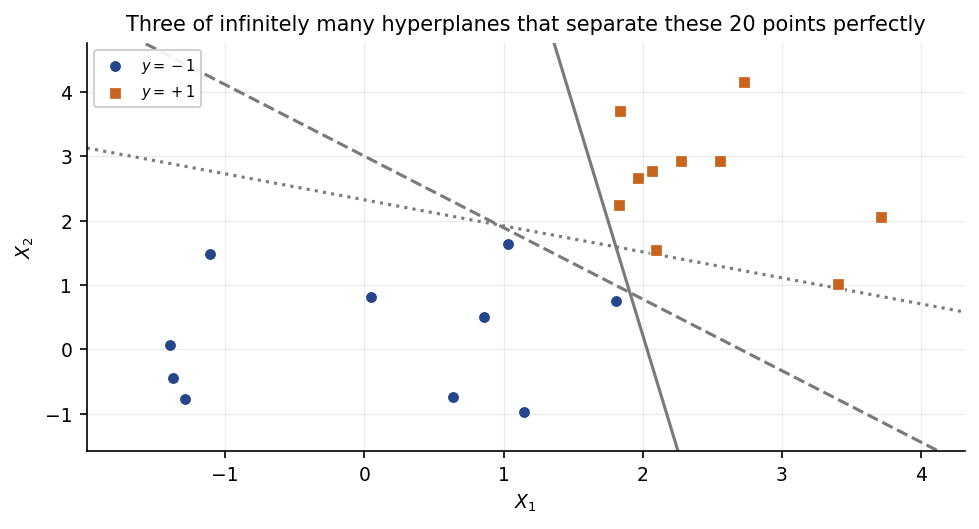
\includegraphics[width=0.88\textwidth,height=0.54\textheight,keepaspectratio]{ch09_many_hyperplanes.png}
  \end{center}
  \begin{takeaway}
    All three lines have zero training error on these $20$ simulated points
    (seed \texttt{2024}), and so do infinitely many others. \textbf{Zero
    training error does not pick a model} --- we need a second criterion.
  \end{takeaway}
\end{frame}

% ------------------------------------------------------------
\begin{frame}{Exercise 9.1 --- Reading a hyperplane [Math]}
\begin{exercise}
  Consider the hyperplane $1 + 2X_1 + 3X_2 = 0$ in $\mathbb{R}^2$ and the rule
  $\hat y = \operatorname{sign}(1+2X_1+3X_2)$.
  \begin{enumerate}
    \item Classify the points $(0,0)$, $(-1,1)$ and $(2,-2)$.
    \item Compute $\|\beta\|$ and the perpendicular distance from each point to
          the hyperplane.
    \item All three coefficients are multiplied by $10$. What happens to the
          predicted classes, and what to the scores $f(x)$?
    \item Which is invariant to that rescaling: the sign of $f$, or its size?
  \end{enumerate}
\end{exercise}
\end{frame}

\begin{frame}{Solution --- Exercise 9.1}
\begin{solutionbox}
  \scriptsize
  \textbf{Method.} Evaluate $f(x)=1+2x_1+3x_2$, read the class off its sign,
  and divide $|f|$ by $\|\beta\|$ to turn the score into a distance.

  \textbf{Parts 1--2.} $\|\beta\|=\sqrt{2^2+3^2}=\sqrt{13}=3.6056$.
  \[
    \begin{array}{l|c|c|c}
      x & f(x) & \hat y & |f(x)|/\|\beta\| \\ \hline
      (0,0)  & 1+0+0 = +1 & +1 & 1/3.6056 = 0.277 \\
      (-1,1) & 1-2+3 = +2 & +1 & 2/3.6056 = 0.555 \\
      (2,-2) & 1+4-6 = -1 & -1 & 1/3.6056 = 0.277
    \end{array}
  \]
  So $(0,0)$ and $(-1,1)$ are on the positive side, $(2,-2)$ on the negative
  side, and $(-1,1)$ is twice as far from the boundary as the other two.

  \textbf{Parts 3--4.} Multiplying by $10$ gives $f\to 10f$ \emph{and}
  $\|\beta\|\to 10\|\beta\|$: every score is ten times larger, but every sign
  --- hence every prediction --- is unchanged, and so is $|f|/\|\beta\|$.
  \textbf{Sign and distance are invariant; the raw score is not.}
\end{solutionbox}
\begin{mistake}
  Reading $|f(x)|$ as a distance without dividing by $\|\beta\|$. The scale of
  $f$ is arbitrary --- which is why the next section \emph{fixes} it by
  demanding $y_i f(x_i)\ge 1$ at the support vectors.
\end{mistake}
\end{frame}

% ============================================================
\section{Maximal Margin}
% ============================================================

\begin{frame}{The margin: the widest street between the classes}
  \footnotesize
  Among all separating hyperplanes, take the one whose nearest training point
  is as far away as possible.
  \begin{block}{The maximal margin problem}
    \[
      \boxed{\;
      \max_{\beta_0,\,\beta,\,M} M
      \quad\text{s.t.}\quad
      \|\beta\| = 1,\qquad
      y_i\big(\beta_0+\beta^\top x_i\big) \ge M \quad \forall\, i=1,\dots,n \;}
    \]
  \end{block}
  \begin{readme}
    \begin{itemize}
      \item $M>0$ is the \textbf{margin}: the perpendicular distance from the
            hyperplane to the closest observation. The street has total width
            $2M$.
      \item The constraint $\|\beta\|=1$ removes the arbitrary scale of
            Exercise 9.1, so $y_i(\beta_0+\beta^\top x_i)$ \emph{is} a signed
            distance.
      \item The $n$ inequalities say: every point is on the correct side
            \emph{and} at least $M$ away.
    \end{itemize}
  \end{readme}
\end{frame}

\begin{frame}{The same problem, in the form software actually solves}
  \footnotesize
  \begin{block}{Equivalent convex form: drop $\|\beta\|=1$, fix the scale instead}
    \[
      \boxed{\;
      \min_{\beta_0,\,\beta}\ \tfrac12\|\beta\|^2
      \quad\text{s.t.}\quad
      y_i\big(\beta_0+\beta^\top x_i\big) \ge 1 \ \ \forall\, i,
      \qquad\text{then}\quad M=\frac{1}{\|\beta\|} \;}
    \]
  \end{block}
  \begin{readme}[Why the two are the same problem]
    \begin{itemize}
      \item Rescale $(\beta_0,\beta)$ so the closest points have
            $y_i f(x_i)=1$ exactly --- the \emph{canonical} scaling.
      \item With that scaling the geometric margin is $1/\|\beta\|$, so
            \emph{maximising} $M$ is \emph{minimising} $\|\beta\|$.
      \item Minimising $\tfrac12\|\beta\|^2$ under linear constraints is a
            convex quadratic programme with a unique solution.
    \end{itemize}
  \end{readme}
  \begin{takeaway}
    ``Widest margin'' $=$ ``smallest coefficients''. This is already a
    ridge-type shrinkage of $\beta$ (Chapter 6); Section 7 makes the penalty
    explicit.
  \end{takeaway}
\end{frame}

\begin{frame}{Support vectors: the only points that matter}
  \begin{center}
    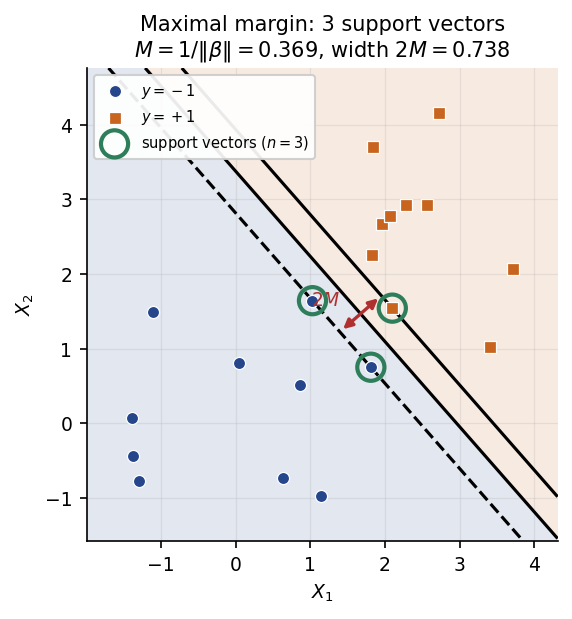
\includegraphics[width=0.38\textwidth,height=0.46\textheight,keepaspectratio]{ch09_maxmargin.png}
  \end{center}
  \begin{takeaway}
    On the seeded data ($n=20$, seed \texttt{2024}), $\|\beta\|=2.711$, so
    $M=1/\|\beta\|=0.369$ and the street is $2M=0.738$ wide. Exactly
    \textbf{three} points touch the kerb ($y_if(x_i)=1$): the \textbf{support
    vectors}. Delete any of the other $17$ and the fit is identical --- they
    carry $\alpha_i=0$ in $f(x)=\beta_0+\sum_i\alpha_i\langle x,x_i\rangle$.
  \end{takeaway}
\end{frame}

\begin{frame}{Fatal flaw 1: with overlapping classes there is no solution}
  \begin{center}
    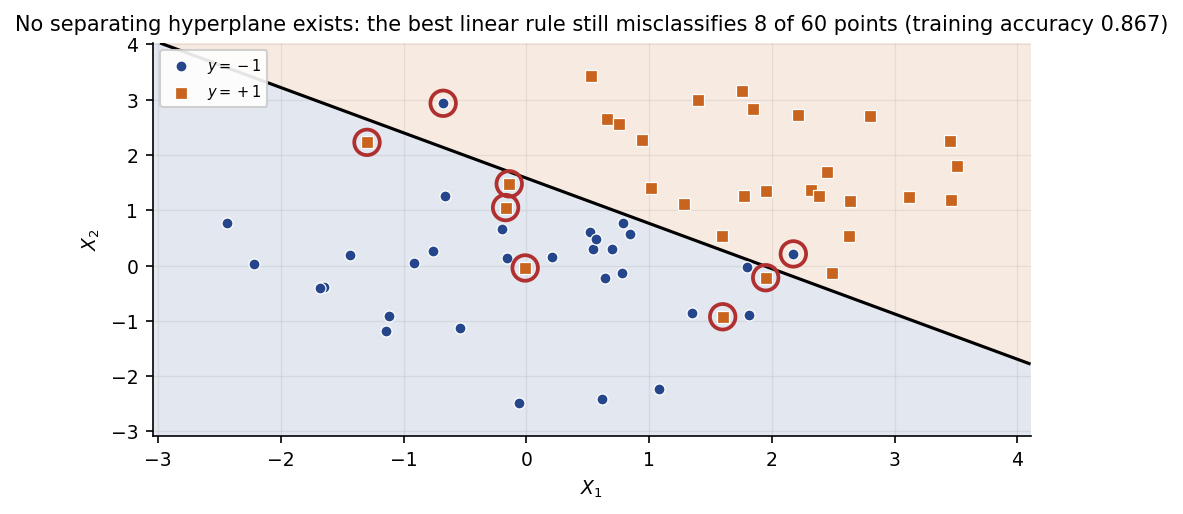
\includegraphics[width=0.82\textwidth,height=0.50\textheight,keepaspectratio]{ch09_nonseparable.png}
  \end{center}
  \begin{takeaway}
    On overlapping data ($n=60$, seed \texttt{2025}) \emph{no} hyperplane
    separates the classes, so the constraint set $y_i f(x_i)\ge M>0$ is
    \textbf{empty} and the problem is infeasible. Even the best linear rule
    misclassifies $8$ of $60$ points (training accuracy $0.867$).
  \end{takeaway}
\end{frame}

\begin{frame}{Fatal flaw 2: one observation dictates the answer}
  \begin{center}
    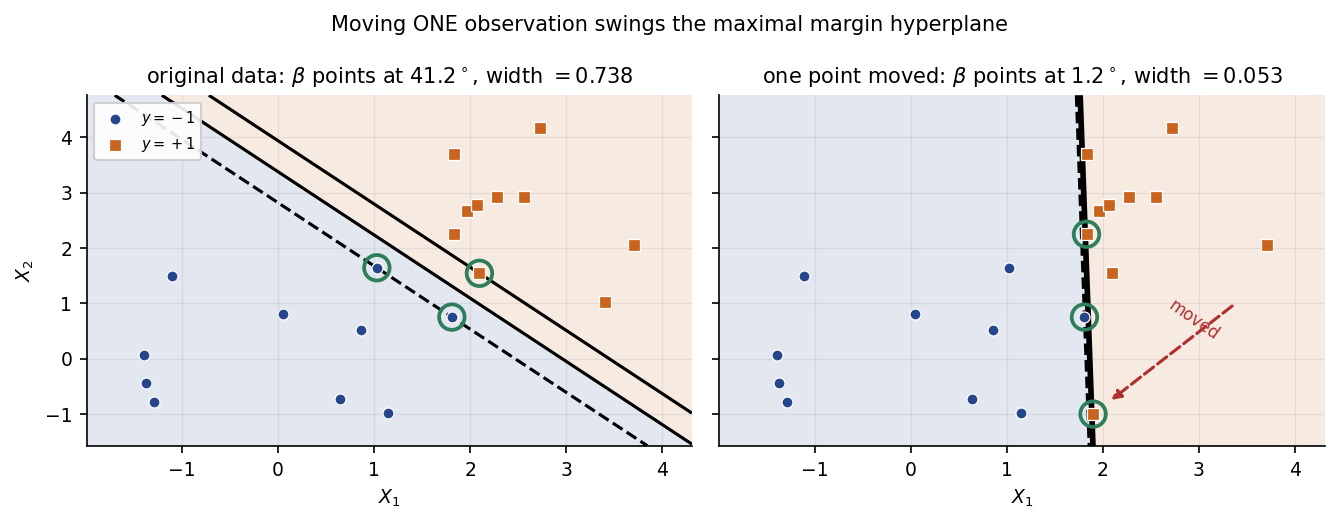
\includegraphics[width=0.94\textwidth,height=0.48\textheight,keepaspectratio]{ch09_instability.png}
  \end{center}
  \begin{takeaway}
    Move a \emph{single} point from $(3.40,\,1.02)$ to $(1.90,\,-1.00)$ --- the
    classes still separate --- and $\beta$ swings from $41.2^\circ$ to
    $1.2^\circ$ while the street collapses from $0.738$ to $0.053$, fourteen
    times narrower. The support vector set changes entirely. That is
    \textbf{variance}, in the Chapter 2 sense.
  \end{takeaway}
\end{frame}

% ------------------------------------------------------------
\begin{frame}{Exercise 9.2 --- The maximal margin by hand [Math]}
\begin{exercise}
  Seven observations in $p=2$, with $y=-1$ and $y=+1$ as shown:
  \[
    \begin{array}{c|ccccccc}
      i & 1 & 2 & 3 & 4 & 5 & 6 & 7\\ \hline
      X_1 & 3 & 2 & 4 & 1 & 2 & 4 & 4\\
      X_2 & 4 & 2 & 4 & 4 & 1 & 3 & 1\\
      y   & -1& -1& -1& -1& +1& +1& +1
    \end{array}
  \]
  \begin{enumerate}
    \item Sketch the points and argue that the optimal separating line is
          $X_2 = X_1 - \tfrac12$.
    \item Write it in canonical form ($y_i f(x_i)\ge 1$, with equality at the
          closest points) and give $\beta_0$, $\beta$, $\|\beta\|$.
    \item Compute the margin $M$ and the street width $2M$.
    \item Which observations are the support vectors? What changes if
          observation $7$ moves to $(4.5,\,0.5)$?
  \end{enumerate}
\end{exercise}
\end{frame}

\begin{frame}{Solution --- Exercise 9.2 (1/2)}
\begin{solutionbox}
  \textbf{Method.} Find the two closest opposite-class pairs, put the boundary
  half-way between them, then rescale so the nearest points score exactly
  $\pm1$.

  \textbf{Part 1.} Along the direction $X_1-X_2$ the classes separate: the
  $y=-1$ points give $X_1-X_2 \in \{-1,0,0,-3\}$, the $y=+1$ points give
  $\{1,1,3\}$. The extremes are $0$ (points $2,3$) and $1$ (points $5,6$), so
  the widest street puts the boundary at the midpoint $X_1-X_2=\tfrac12$,
  i.e.\ $X_2=X_1-\tfrac12$.

  \textbf{Part 2.} With $g(x)= -\tfrac12 + x_1 - x_2$ we get
  $g=\mp\tfrac12$ at the four closest points, so multiply by $2$:
  \[
    f(x) = -1 + 2x_1 - 2x_2,
    \quad \beta_0=-1,\quad \beta=(2,-2)^\top,\quad
    \|\beta\|=2\sqrt2 = 2.8284 .
  \]
  Check: $f(2,2)=-1$, $f(4,4)=-1$, $f(2,1)=+1$, $f(4,3)=+1$, so
  $y_if(x_i)=1$ there, while $f(3,4)=-3$, $f(1,4)=-7$, $f(4,1)=+5$ give
  $y_if(x_i)>1$.
\end{solutionbox}
\end{frame}

\begin{frame}{Solution --- Exercise 9.2 (2/2)}
\begin{solutionbox}
  \scriptsize
  \textbf{Part 3.}
  $M=1/\|\beta\|=1/(2\sqrt2)=0.3536$ and $2M = 1/\sqrt2 = 0.7071$.

  \textbf{Part 4.} The support vectors are the four points with
  $y_if(x_i)=1$: observations $2\,(2,2)$ and $3\,(4,4)$ from the $-1$ class,
  $5\,(2,1)$ and $6\,(4,3)$ from the $+1$ class. Observations $1$, $4$, $7$
  are strictly outside the street.

  Moving observation $7$ from $(4,1)$ to $(4.5,0.5)$ takes it \emph{further}
  away ($f$ goes from $+5$ to $+7$), so it is still not a support vector: the
  hyperplane, the margin and the fit are \textbf{completely unchanged}.

  \textit{Note for the lab:} \texttt{SVC(kernel='linear', C=1e6)} recovers
  $\beta\approx(2,-2)$, $\beta_0\approx-1$, but may list only \emph{three}
  entries in \texttt{support\_}: with four points tied on the margin the dual
  solution is not unique and one multiplier can be exactly zero. All four are
  still support vectors geometrically.
\end{solutionbox}
\begin{mistake}
  Putting the boundary through the midpoint of the two class \emph{centroids}.
  The margin is set by the \emph{closest} pair; interior points are irrelevant.
\end{mistake}
\end{frame}

% ============================================================
\section{Soft Margin}
% ============================================================

\begin{frame}{Buying robustness with violations}
  \footnotesize
  Both flaws have one cure: stop insisting that every point be correct, and
  \emph{pay} for the exceptions.
  \begin{block}{The support vector classifier (ISLP form)}
    \[
      \boxed{\;
      \max_{\beta_0,\beta,\xi,M} M
      \ \text{ s.t. }\
      \|\beta\|=1,\quad
      y_i f(x_i)\ge M(1-\xi_i),\quad
      \xi_i\ge0,\quad \sum_{i=1}^n \xi_i \le C_{\text{ISLP}} \;}
    \]
  \end{block}
  \begin{readme}[Read every symbol]
    \begin{itemize}
      \item $\xi_i$ is the \textbf{slack} of observation $i$, measured in units
            of the margin $M$.
      \item $M$ is still \emph{maximised}; what is \emph{budgeted} is the
            \textbf{sum of the slacks}, $\sum_i\xi_i \le C_{\text{ISLP}}$ ---
            not the number of violations, and not each $\xi_i$ separately.
      \item $C_{\text{ISLP}}=0$ forces every $\xi_i=0$: the hard margin is the
            special case. Because it is a \emph{total} budget, one badly placed
            point can eat the whole allowance alone.
    \end{itemize}
  \end{readme}
\end{frame}

\begin{frame}{What each slack value means}
  \scriptsize
  \begin{center}
  \begin{tabular}{@{}lll@{}}
    \toprule
    \textbf{Slack} & \textbf{Where the point sits} & \textbf{Support vector?} \\
    \midrule
    $\xi_i = 0$, $y_if(x_i)>1$ & strictly outside the street & no --- irrelevant to the fit \\
    $\xi_i = 0$, $y_if(x_i)=1$ & exactly on the kerb & yes \\
    $0 < \xi_i \le 1$ & inside the street, still on its own side & yes \\
    $\xi_i > 1$ & on the \emph{wrong} side --- misclassified & yes \\
    \bottomrule
  \end{tabular}
  \end{center}
  \begin{center}
    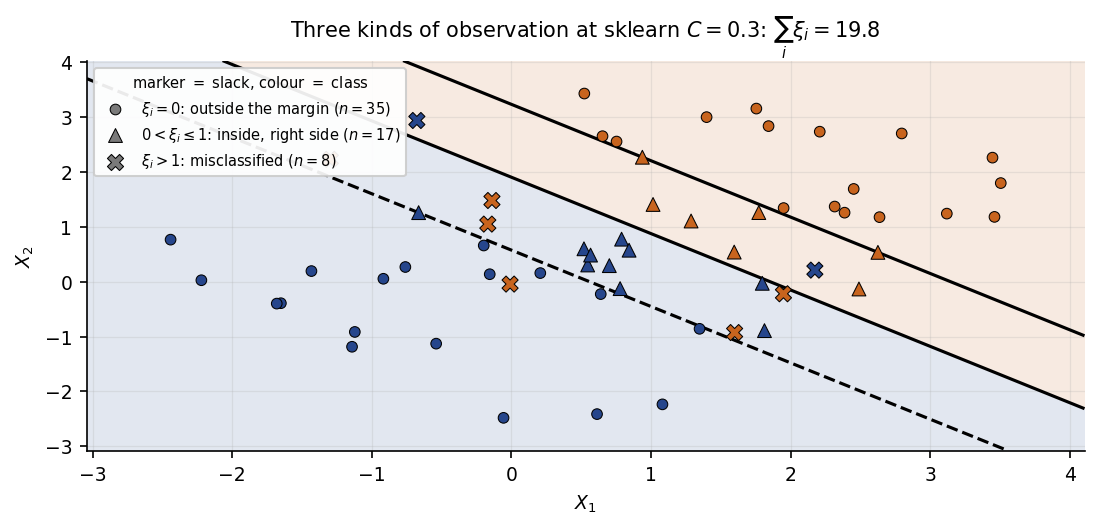
\includegraphics[width=0.62\textwidth,height=0.36\textheight,keepaspectratio]{ch09_slack_anatomy.png}
  \end{center}
  \begin{takeaway}
    Marker shape is the slack category, colour the class. At sklearn $C=0.3$:
    $35$ points outside the street, $17$ inside it on their own side, $8$
    misclassified, total $\sum_i\xi_i = 19.8$.
  \end{takeaway}
\end{frame}

\begin{frame}{The form scikit-learn solves --- and the trap}
  \footnotesize
  \begin{block}{Hinge-loss form (this is what \texttt{SVC} minimises)}
    \[
      \boxed{\;
      \min_{\beta_0,\beta,\xi}\ \tfrac12\|\beta\|^2 + C\sum_{i=1}^{n}\xi_i
      \quad\text{s.t.}\quad
      y_i f(x_i)\ge 1-\xi_i,\quad \xi_i\ge0 \;}
    \]
  \end{block}
  \begin{readme}[Where the inversion comes from]
    Divide by $C$: the objective is $\tfrac{1}{2C}\|\beta\|^2 + \sum_i \xi_i$,
    so the ridge penalty weight is $\lambda = 1/(2C)$.
    \textbf{Large $C$} $\Rightarrow$ violations expensive $\Rightarrow$
    $\|\beta\|$ free to grow $\Rightarrow$ \textbf{narrow} margin, \emph{less}
    regularisation. \textbf{Small $C$} $\Rightarrow$ the reverse.
  \end{readme}
  \begin{mistake}[The single most common source of confusion in this chapter]
    ISLP's $C_{\text{ISLP}}$ is a \emph{budget for violations}: large budget
    $=$ wide margin. Scikit-learn's $C$ is a \emph{cost per violation}: large
    $C$ $=$ \textbf{narrow} margin. The conventions run in \textbf{opposite}
    directions, roughly $C \sim 1/C_{\text{ISLP}}$. Get it backwards and your
    whole bias--variance story inverts.
  \end{mistake}
\end{frame}

\begin{frame}{The two conventions side by side}
  \scriptsize
  \begin{center}
  \begin{tabular}{@{}p{3.2cm}p{4.1cm}p{4.1cm}@{}}
    \toprule
     & \textbf{ISLP $C_{\text{ISLP}}$} (a budget) & \textbf{sklearn $C$} (a cost) \\
    \midrule
    Appears in & $\sum_i \xi_i \le C_{\text{ISLP}}$ & $+\,C\sum_i \xi_i$ in the objective \\
    Larger value means & more violations \emph{allowed} & each violation \emph{more expensive} \\
    Margin & wider & narrower \\
    Support vectors & more & fewer \\
    Flexibility & lower (more bias) & higher (more variance) \\
    Hard margin at & $C_{\text{ISLP}}=0$ & $C\to\infty$ \\
    \bottomrule
  \end{tabular}
  \end{center}
  \begin{takeaway}
    Whenever you read ``increase $C$'', check \emph{whose} $C$. Every slide
    here that says ``sklearn $C$'', and every line of notebook code, uses the
    scikit-learn convention: \textbf{big $C$, narrow street}. Write the library
    and version next to any reported value --- ``$C=100$, a highly regularised
    model'' is the sentence that gets a validation report sent back.
  \end{takeaway}
\end{frame}

\begin{frame}{$C$ is the bias--variance dial (bridge to Chapter 2)}
  \begin{center}
    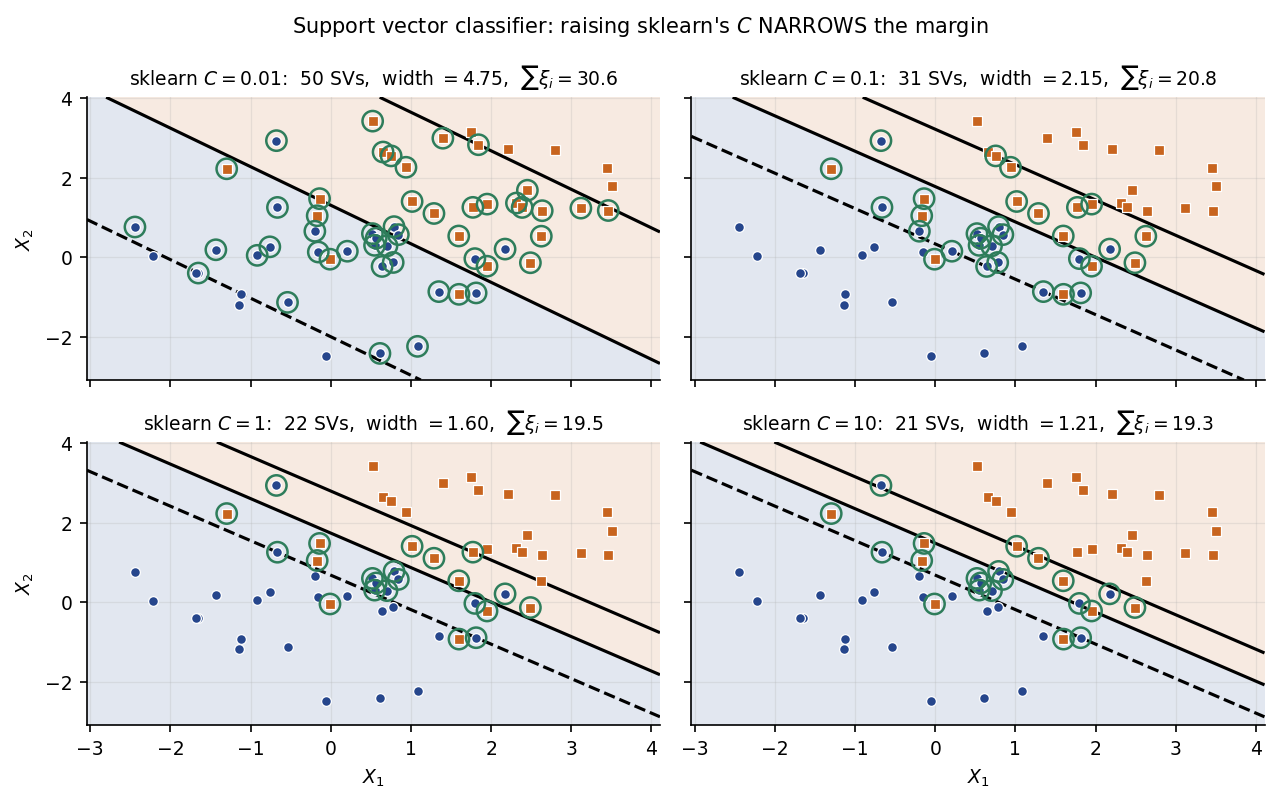
\includegraphics[width=0.62\textwidth,height=0.46\textheight,keepaspectratio]{ch09_soft_C.png}
  \end{center}
  \begin{takeaway}
    As sklearn $C$ rises $0.01\to10$ on the same $60$ points: street width
    falls $4.75\to1.21$, support vectors fall $50\to21$, $\sum_i\xi_i$ falls
    $30.6\to19.3$. A wide margin rests on many points, so no single one can
    move it --- low variance, high bias. Training accuracy is not even monotone
    ($0.850$, $0.867$, $0.867$, $0.850$): tune $C$ by \textbf{cross-validation}.
  \end{takeaway}
\end{frame}

% ------------------------------------------------------------
\begin{frame}{Exercise 9.3 --- Slacks, budgets and sklearn's $C$ [Concept]}
\begin{exercise}
  \begin{enumerate}
    \item State precisely what is maximised and what is constrained in the
          support vector classifier. Which quantity carries the budget?
    \item An observation has $\xi_i = 0.4$. Where is it, and is it a support
          vector? Repeat for $\xi_i = 1.8$.
    \item A colleague reports: ``I raised \texttt{SVC(C=...)} from $0.1$ to
          $100$ to regularise the model more strongly.'' What is wrong, and
          what actually happened to the margin and to $|\mathcal S|$?
    \item You fit a support vector classifier to $n=200$ points and find $196$
          support vectors. What does that say about $C$ and about the
          bias--variance position of the fit?
  \end{enumerate}
\end{exercise}
\end{frame}

\begin{frame}{Solution --- Exercise 9.3}
\begin{solutionbox}
  \scriptsize
  \textbf{Part 1.} The \emph{margin} $M$ is maximised, under
  $y_i f(x_i)\ge M(1-\xi_i)$ with $\xi_i\ge0$; the budget sits on the
  \textbf{sum} of the slacks, $\sum_{i=1}^n \xi_i \le C_{\text{ISLP}}$ --- not
  on each $\xi_i$, and not on a count of violations.

  \textbf{Part 2.} $\xi_i=0.4\in(0,1]$: inside the street but still on the
  correct side. $\xi_i=1.8>1$: on the wrong side, \emph{misclassified}. Both
  have $y_if(x_i)\le1$, so \textbf{both are support vectors}.

  \textbf{Part 3.} The direction is inverted. In scikit-learn $C$ is the
  \emph{cost per unit slack} in $\tfrac12\|\beta\|^2 + C\sum_i\xi_i$, i.e.\
  penalty weight $\lambda=1/(2C)$. Raising $C$ from $0.1$ to $100$
  \textbf{weakens} regularisation: slacks shrink, $\|\beta\|$ grows, the margin
  $1/\|\beta\|$ \emph{narrows}, $|\mathcal S|$ \emph{falls}. The model became
  \emph{more} flexible --- the opposite of the stated intent.

  \textbf{Part 4.} $196$ of $200$ points have $y_if(x_i)\le1$, so nearly the
  whole sample lies inside a very wide street: a \textbf{small} $C$ (large
  ISLP budget), heavily regularised, high bias, low variance. If CV accuracy is
  poor, raise $C$; if it is already good, the wide margin is buying stability
  for free.
\end{solutionbox}
\begin{mistake}
  Treating many support vectors as evidence of overfitting. It is the opposite
  signal: many support vectors means a wide margin, hence a smooth, heavily
  regularised fit.
\end{mistake}
\end{frame}

% ------------------------------------------------------------
% EXTENDED EXERCISE 9.1
\begin{frame}{Extended Exercise 9.1 --- From hard to soft margin by hand [Math]}
\begin{longexercise}
  Take the seven points of Exercise 9.2 with the hard-margin solution
  $f(x)=-1+2x_1-2x_2$, $\|\beta\|=2\sqrt2$, $M=0.3536$.
  \begin{enumerate}
    \item Add an eighth observation at $(2,3)$ with $y_8=+1$. Show that the
          data are no longer separable, so the hard-margin problem is
          infeasible.
    \item Keeping the \emph{same} $f$, compute
          $\xi_i = \max\{0,\,1-y_i f(x_i)\}$ for all eight points and the total
          $\sum_i \xi_i$.
    \item How large must $C_{\text{ISLP}}$ be for this $f$ to be feasible?
          Which observations are now support vectors?
    \item In terms of $\tfrac12\|\beta\|^2 + C\sum_i\xi_i$, what would a
          \emph{small} sklearn $C$ do to this fit instead?
  \end{enumerate}
\end{longexercise}
\end{frame}

\begin{frame}{Solution --- Extended Exercise 9.1 (1/2)}
\begin{solutionbox}[{{Solution --- parts 1 and 2: separability, and the slacks}}]
  \scriptsize
  \textbf{Part 1.} The new point $(2,3)$ has $x_1-x_2=-1$, the same value as
  observation $1$ at $(3,4)$ --- but observation $1$ has $y=-1$ and the new
  point $y=+1$. Along that direction the classes now overlap; in fact the
  convex hulls of the two classes intersect. Two intersecting convex sets
  cannot be separated by a hyperplane, so no $(\beta_0,\beta)$ satisfies
  $y_if(x_i)\ge M>0$ for all $i$: the programme is \textbf{infeasible}.

  \textbf{Part 2.} With $f(x)=-1+2x_1-2x_2$:
  \[
    \begin{array}{c|cccccccc}
      i & 1 & 2 & 3 & 4 & 5 & 6 & 7 & 8\\ \hline
      x & (3,4) & (2,2) & (4,4) & (1,4) & (2,1) & (4,3) & (4,1) & (2,3)\\
      y_i & -1 & -1 & -1 & -1 & +1 & +1 & +1 & +1\\
      f(x_i) & -3 & -1 & -1 & -7 & +1 & +1 & +5 & -3\\
      y_i f(x_i) & 3 & 1 & 1 & 7 & 1 & 1 & 5 & -3\\
      \xi_i & 0 & 0 & 0 & 0 & 0 & 0 & 0 & 4
    \end{array}
  \]
  Only the new point violates anything, and it violates a lot:
  $\xi_8 = 1-(-3) = 4$, so $\sum_{i=1}^{8}\xi_i = 4$. \textbf{One badly placed
  observation consumes the entire budget} --- the honest reading of ``the budget
  is on the \emph{sum} of the slacks''.
\end{solutionbox}
\end{frame}

\begin{frame}{Solution --- Extended Exercise 9.1 (2/2)}
\begin{solutionbox}[{{Solution --- parts 3 and 4: budget, support vectors, sklearn's $C$}}]
  \scriptsize
  \textbf{Part 3.} This $f$ becomes feasible as soon as
  $C_{\text{ISLP}} \ge \sum_i \xi_i = 4$. The support vectors are every point
  with $y_i f(x_i)\le 1$: observations $2, 3, 5, 6$ (on the kerb, $\xi=0$) and
  observation $8$ (misclassified, $\xi_8=4$) --- five in all. Observations
  $1$, $4$, $7$ remain irrelevant.

  \textbf{Part 4.} In the scikit-learn objective this $f$ costs
  $\tfrac12(2\sqrt2)^2 + 4C = 4 + 4C$. With a \emph{small} $C$ the $4C$ term is
  cheap, so the solver buys more slack in exchange for a smaller $\|\beta\|$:
  it tilts and \emph{widens} the street, lets several points drift inside, and
  becomes smoother and far less sensitive to point $8$. With a \emph{large} $C$
  it contorts to keep $\xi_8$ small, ending up with a large $\|\beta\|$ and a
  narrow, unstable margin.
\end{solutionbox}
\begin{mistake}
  Computing $\xi_8$ as a geometric distance. The slack lives on the
  \emph{functional} margin scale, $\xi_i=\max\{0,1-y_if(x_i)\}$, so it is $4$
  here --- not $4/\|\beta\| = 1.41$.
\end{mistake}
\end{frame}

% ============================================================
\section{Kernels}
% ============================================================

\begin{frame}{When no straight line will do}
  \begin{center}
    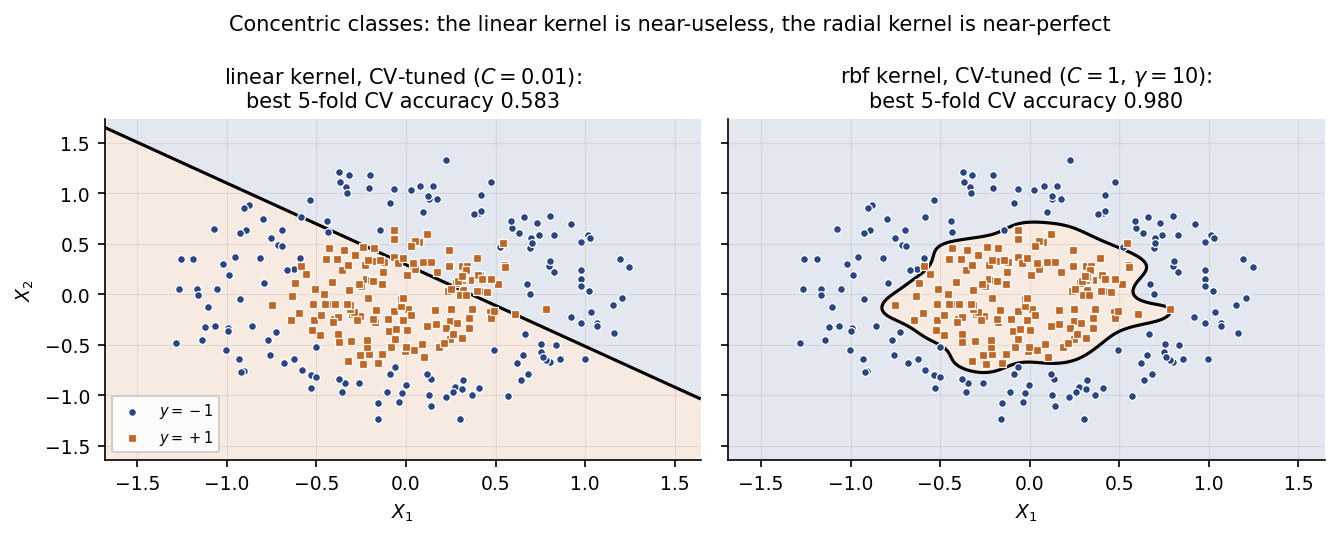
\includegraphics[width=0.86\textwidth,height=0.48\textheight,keepaspectratio]{ch09_nonlinear_fail.png}
  \end{center}
  \begin{takeaway}
    $300$ points on two concentric rings (\texttt{make\_circles},
    \texttt{random\_state=0}). Even with $C$ chosen by 5-fold CV the
    \textbf{linear} kernel reaches only $0.583$ accuracy --- barely above the
    $0.500$ coin flip --- while the radial kernel reaches $0.980$. No amount of
    soft-margin tuning fixes a wrong \emph{shape}.
  \end{takeaway}
\end{frame}

\begin{frame}{The old trick: enlarge the feature space}
  \footnotesize
  Chapter 7's answer: add non-linear columns and fit a \emph{linear} rule in
  the bigger space.
  \begin{numexample}[{{The concentric data, made separable}}]
    Add one feature, $X_3 = X_1^2 + X_2^2$. In $(X_1,X_2,X_3)$-space the inner
    ring sits at small $X_3$, the outer at large $X_3$, so the plane $X_3 = c$
    separates them perfectly. A curved boundary in $\mathbb{R}^2$ is a flat one
    in $\mathbb{R}^3$.
  \end{numexample}
  \begin{readme}[Why this does not scale]
    All monomials up to degree $d$ in $p$ predictors number
    $\binom{p+d}{d}$. With $p=100$, $d=3$ that is $176\,851$ columns; at $d=4$,
    over four million. We cannot build, store or fit that design matrix.
  \end{readme}
  \begin{takeaway}
    The kernel trick delivers the enlarged space \emph{without ever
    constructing it}.
  \end{takeaway}
\end{frame}


\begin{frame}{What the enlargement costs, drawn}
  \begin{center}
    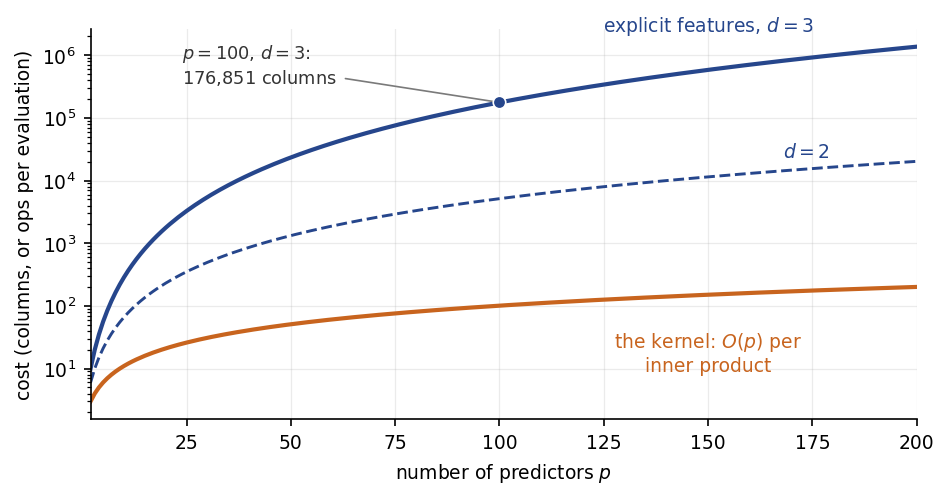
\includegraphics[width=0.74\textwidth,height=0.54\textheight,keepaspectratio]{ch09_feature_blowup.png}
  \end{center}
  \begin{takeaway}
    Monomials up to degree $d$ in $p$ variables: $\binom{p+d}{d}$ columns.
    At $p=100$, $d=3$ the explicit design matrix has $176\,851$ columns; the
    kernel computes the \emph{same} inner product in $O(p)$ operations. That
    gap is the kernel trick.
  \end{takeaway}
\end{frame}

\begin{frame}{The kernel trick}
  \scriptsize
  \begin{block}{From inner products to kernels}
    \[
      \boxed{\;
      f(x) = \beta_0 + \sum_{i=1}^{n}\alpha_i\,\langle x, x_i\rangle
      \ \longrightarrow\
      f(x) = \beta_0 + \sum_{i\in\mathcal S}\alpha_i\, K(x, x_i),
      \quad K(x,x') = \langle \phi(x), \phi(x')\rangle \;}
    \]
  \end{block}
  \begin{readme}
    \begin{itemize}
      \item Fitting \emph{and} prediction touch the data only through pairwise
            inner products. Replace that one function and you have replaced the
            feature space.
      \item A \textbf{kernel} $K$ is any similarity that equals an inner
            product in \emph{some} enlarged space $\phi(\cdot)$; symmetric and
            positive semi-definite suffices, and we never need to know $\phi$.
      \item $\alpha_i = 0$ off the support vectors, so the stored model is
            small. A support vector classifier with a non-linear kernel is a
            \textbf{support vector machine}.
    \end{itemize}
  \end{readme}
  \begin{takeaway}
    Cost is set by $n$ (an $n\times n$ kernel matrix), not by the dimension of
    the enlarged space --- which may be infinite.
  \end{takeaway}
\end{frame}

\begin{frame}{The three kernels you will actually use}
  \footnotesize
  \begin{block}{Definitions}
    \[
      \underbrace{\langle x, x'\rangle}_{\text{linear}}
      \qquad
      \underbrace{\big(1+\langle x, x'\rangle\big)^{d}}_{\text{polynomial},\ d=1,2,3,\dots}
      \qquad
      \underbrace{\exp\!\big(-\gamma\,\|x-x'\|^2\big)}_{\text{radial (RBF)},\ \gamma>0}
    \]
  \end{block}
  \begin{readme}[What each buys]
    \begin{itemize}
      \item \textbf{Linear} ($d=1$) reproduces the support vector classifier;
            the right default when $p$ is large.
      \item \textbf{Polynomial} of degree $d$ spans all monomials up to degree
            $d$; ill-behaved numerically for $d\ge4$ and rarely worth it.
      \item \textbf{Radial} corresponds to an \emph{infinite}-dimensional
            $\phi$ and is the workhorse: \texttt{kernel='rbf'}, parameter
            \texttt{gamma}.
    \end{itemize}
  \end{readme}
  \begin{mistake}
    \texttt{SVC(kernel='poly', degree=2)} does \emph{not} match the formula
    above: sklearn uses $(\gamma\langle x,x'\rangle + r)^d$ with
    $r=$\texttt{coef0}$=0$ by default, which kills the lower-order terms. Set
    \texttt{coef0=1} (and \texttt{gamma=1}) for ISLP's kernel.
  \end{mistake}
\end{frame}

\begin{frame}{The radial kernel: $\gamma$ sets how local the boundary is}
  \footnotesize
  \begin{block}{Reading the radial kernel}
    \[
      \boxed{\;K(x,x') = \exp\!\big(-\gamma\|x-x'\|^2\big) \in (0,1] \;}
    \]
  \end{block}
  \begin{readme}
    \begin{itemize}
      \item $K$ equals $1$ when $x=x'$ and decays towards $0$ as the points
            separate; $\gamma$ sets \emph{how fast}.
      \item \textbf{Small $\gamma$}: distant points still count, every support
            vector votes everywhere, the boundary is smooth and nearly linear
            --- high bias.
      \item \textbf{Large $\gamma$}: only near neighbours count, so each
            support vector carves out its own island --- high variance. The
            limit is a nearest-neighbour rule.
      \item $\|x-x'\|^2$ is a \emph{squared distance}, so $\gamma$ carries
            units of $1/\text{(distance)}^2$: it is meaningless without a fixed
            scale for the predictors.
    \end{itemize}
  \end{readme}
\end{frame}

\begin{frame}{What $\gamma$ does to the boundary}
  \begin{center}
    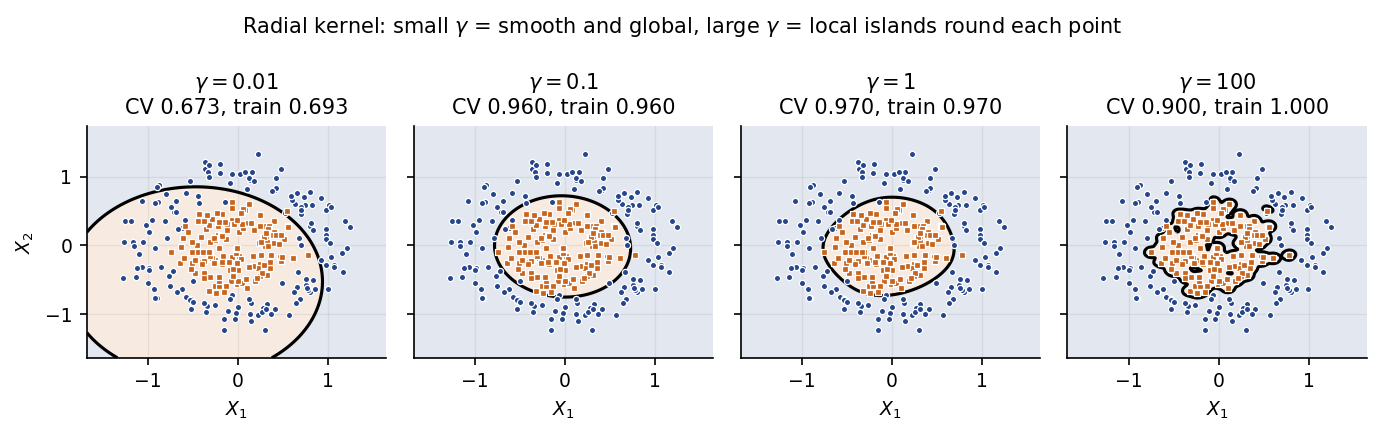
\includegraphics[width=0.96\textwidth,height=0.42\textheight,keepaspectratio]{ch09_gamma.png}
  \end{center}
  \begin{takeaway}
    At $C=1$ on the concentric data: $\gamma=0.01$ is too smooth to see the
    ring at all (CV $0.673$); $\gamma=0.1$ and $1$ recover it ($0.960$,
    $0.970$); $\gamma=100$ fits the training set \emph{perfectly} ($1.000$) by
    growing islands round individual points, and CV accuracy \emph{drops} to
    $0.900$. Textbook overfitting.
  \end{takeaway}
\end{frame}

\begin{frame}{$C$ and $\gamma$ pull on the same rope}
  \begin{readme}[{{Two knobs, one flexibility}}]
    \begin{itemize}
      \item $\gamma$ controls the \emph{shape}: how wiggly the boundary may be.
      \item sklearn's $C$ controls how hard the fit \emph{insists} that this
            shape reproduce the training labels.
      \item Large $\gamma$ \emph{and} large $C$ is the fastest route to a
            memorised training set; small $\gamma$ \emph{and} small $C$ is
            almost a linear rule.
    \end{itemize}
  \end{readme}
  \begin{takeaway}
    They interact, so they must be tuned \textbf{jointly} on a grid, never one
    after the other. And because $\gamma$ is tied to the \emph{scale} of the
    features, a fitted pair $(C,\gamma)$ is only valid alongside the scaler it
    was tuned with: freeze the two together and re-tune on a schedule.
  \end{takeaway}
\end{frame}

\begin{frame}{Scaling is not optional}
  \footnotesize
  \begin{numexample}[Heart data: what unscaled predictors do to a radial kernel]
    The $16$ predictors have wildly different spreads --- \texttt{Chol} has
    standard deviation $52.0$, \texttt{Fbs} has $0.35$. The median squared
    distance between two patients is $\|x-x'\|^2 \approx 4\,294$ raw against
    $31.1$ standardised, so at $\gamma=0.05$ a typical kernel entry is
    $e^{-0.05\times 4294} = 5.8\times10^{-94}$ raw against $0.211$
    standardised. The raw kernel matrix is numerically the identity.
  \end{numexample}
  \begin{takeaway}
    On the Heart test set the identical model (\texttt{rbf}, $C=1$,
    $\gamma=0.05$) scores $0.556$ unscaled and $\mathbf{0.822}$ scaled.
    Unscaled it predicts ``No'' for $86$ of $90$ test patients --- it has
    collapsed to the majority class.
  \end{takeaway}
  \begin{mistake}
    Standardising \emph{before} the train/test split, or outside the
    cross-validation loop. Put \texttt{StandardScaler} inside a
    \texttt{Pipeline} so every fold rescales with its own training rows only.
  \end{mistake}
\end{frame}

% ------------------------------------------------------------
\begin{frame}{Exercise 9.4 --- The polynomial kernel is an inner product [Math]}
\begin{exercise}
  Let $p=2$ and $K(x,x') = \big(1+\langle x,x'\rangle\big)^2$ with
  $x=(x_1,x_2)$, $x'=(x'_1,x'_2)$.
  \begin{enumerate}
    \item Expand $K(x,x')$ fully in the four coordinates.
    \item Exhibit an explicit map $\phi:\mathbb{R}^2\to\mathbb{R}^m$ with
          $K(x,x')=\langle\phi(x),\phi(x')\rangle$. What is $m$?
    \item How many multiplications does each route need for one kernel entry?
    \item The enlarged space has $\binom{p+d}{d}$ dimensions. Evaluate this for
          $p=100$, $d=3$, and state the cost of the kernel route instead.
  \end{enumerate}
\end{exercise}
\end{frame}

\begin{frame}{Solution --- Exercise 9.4 (1/2)}
\begin{solutionbox}
  \scriptsize
  \textbf{Part 1.} With $s = x_1x'_1 + x_2x'_2$,
  \[
    K = (1+s)^2 = 1 + 2s + s^2
      = 1 + 2x_1x'_1 + 2x_2x'_2 + x_1^2x'^2_1 + x_2^2x'^2_2
        + 2x_1x_2x'_1x'_2 .
  \]

  \textbf{Part 2.} Read the six terms as one inner product, splitting each
  factor $2$ as $\sqrt2\cdot\sqrt2$:
  \[
    \phi(x) = \big(1,\ \sqrt2\,x_1,\ \sqrt2\,x_2,\ x_1^2,\ x_2^2,\
                    \sqrt2\,x_1x_2\big) \in \mathbb{R}^6,
    \qquad m = 6 = \binom{4}{2}. \ \checkmark
  \]
\end{solutionbox}
\end{frame}

\begin{frame}{Solution --- Exercise 9.4 (2/2)}
\begin{solutionbox}
  \textbf{Part 3.} Via the kernel: two products for $s$, then one squaring ---
  \textbf{three} multiplications. Via $\phi$: \textbf{six} multiplications for
  the inner product, plus building both $6$-vectors and storing $6$ numbers per
  observation instead of $2$.

  \textbf{Part 4.}
  $\binom{103}{3} = (103\cdot102\cdot101)/6 = 176\,851$ columns in the enlarged
  design matrix, versus $p+1 = 101$ multiplications per pair for the kernel and
  no extra storage --- the \emph{same fit} at a cost independent of the
  enlarged dimension.
\end{solutionbox}
\begin{mistake}
  Dropping the $\sqrt2$ factors and writing
  $\phi(x)=(1,x_1,x_2,x_1^2,x_2^2,x_1x_2)$. That map reproduces the cross
  terms with the wrong weights, so it is a \emph{different} kernel.
\end{mistake}
\end{frame}

% ------------------------------------------------------------
\begin{frame}{Exercise 9.5 --- Kernels on the concentric data [Python]}
\begin{exercise}
  Generate \texttt{X, y = make\_circles(n\_samples=300, factor=0.4,
  noise=0.15, random\_state=0)}.
  \begin{enumerate}
    \item In a \texttt{Pipeline} with \texttt{StandardScaler}, tune a
          \textbf{linear} SVM over \texttt{C = np.logspace(-2, 2, 9)} by
          5-fold CV. Report the best $C$ and CV accuracy.
    \item Tune a \textbf{radial} SVM over \texttt{C = np.logspace(-2, 2, 5)}
          and \texttt{gamma = np.logspace(-3, 1, 5)}.
    \item Fit a \textbf{polynomial} kernel of degree $2$ with
          \texttt{coef0=1, C=1}. Does it match the radial kernel?
    \item Explain the gap between (1) and (2) in one sentence.
  \end{enumerate}
\end{exercise}
\begin{labnote}[Run this live]
  The worked solution sits in \texttt{advanced\_05\_svm\_lab.ipynb} under
  \emph{Lecture exercises --- worked Python solutions}: the cell headed
  \emph{Exercise 9.5 --- Kernels on the concentric data [Python]}.
\end{labnote}
\end{frame}

\begin{frame}[fragile]{Solution --- Exercise 9.5 (1/2)}
\begin{solutionbox}[Solution --- code]
\begin{lstlisting}[basicstyle=\ttfamily\tiny]
import numpy as np
from sklearn.datasets import make_circles        # rings: no line works
from sklearn.model_selection import GridSearchCV, cross_val_score  # tune / score
from sklearn.pipeline import make_pipeline
from sklearn.preprocessing import StandardScaler  # kernels need one scale
from sklearn.svm import SVC

X, y = make_circles(n_samples=300, factor=0.4, noise=0.15, random_state=0)
pipe = lambda **kw: make_pipeline(StandardScaler(), SVC(**kw))  # scale, then fit

lin = GridSearchCV(pipe(kernel='linear'),                        # (1) linear
                   {'svc__C': np.logspace(-2, 2, 9)}, cv=5).fit(X, y)  # 9 C values
rbf = GridSearchCV(pipe(kernel='rbf'),                           # (2) radial
                   {'svc__C': np.logspace(-2, 2, 5),
                    'svc__gamma': np.logspace(-3, 1, 5)}, cv=5).fit(X, y)  # 25 cells
pol = cross_val_score(pipe(kernel='poly', degree=2, coef0=1, C=1), X, y, cv=5)

print('linear', lin.best_params_, round(lin.best_score_, 3))   # 0.583: coin flip
print('radial', rbf.best_params_, round(rbf.best_score_, 3))   # 0.980: shape fixed
print('poly d=2  CV', round(pol.mean(), 3))   # 0.963: a circle is degree 2
\end{lstlisting}
{\scriptsize\textbf{Reading it:} one \texttt{Pipeline} per kernel, one 5-fold
CV --- each line prints the winning cell and its CV accuracy.}
\end{solutionbox}
\end{frame}

\begin{frame}{Solution --- Exercise 9.5 (2/2)}
\begin{solutionbox}[{{Solution --- output, and how to read it}}]
  \scriptsize
  \textbf{Printout.}
  \begin{center}\ttfamily\scriptsize
  linear \{'svc\_\_C': 0.01\} 0.583 \quad radial \{'svc\_\_C': 1.0, 'svc\_\_gamma': 10.0\} 0.98
  \quad poly d=2 \ CV 0.963
  \end{center}
  \begin{itemize}
    \item \textbf{(1)} The best linear SVM reaches $0.583$; with a $50/50$
          class split that is barely better than a coin flip. Note CV picked
          the \emph{smallest} $C$: when no line can work, a wide margin at
          least keeps the fit stable.
    \item \textbf{(2)} The radial kernel reaches $\mathbf{0.980}$ at $C=1$,
          $\gamma=10$ --- a $0.40$ jump in accuracy from one change of kernel.
    \item \textbf{(3)} Degree $2$ scores $0.963$, and that is no accident: the
          true boundary is a circle, exactly a degree-$2$ surface. The radial
          kernel wins slightly because it can also absorb noise in the ring's
          radius.
    \item \textbf{(4)} The classes are \emph{concentric}, so no half-space
          contains one class: the failure is the boundary's \emph{shape}, and
          only a change of kernel --- not of $C$ --- can fix it.
  \end{itemize}
\end{solutionbox}
\end{frame}

% ------------------------------------------------------------
\begin{frame}{Exercise 9.6 --- Scaling the Heart predictors [Python]}
\begin{exercise}
  Load \texttt{Heart.csv} with \texttt{index\_col=0}, drop rows with missing
  values, code \texttt{AHD} as $0/1$, one-hot encode \texttt{ChestPain} and
  \texttt{Thal} with \texttt{drop\_first=True}, and split with
  \texttt{test\_size=0.3, random\_state=0}.
  \begin{enumerate}
    \item Fit \texttt{SVC(kernel='rbf', C=1, gamma=0.05)} on the \emph{raw}
          predictors; report the test accuracy and the class counts it predicts.
    \item Fit the same model inside
          \texttt{make\_pipeline(StandardScaler(), ...)} and report the test
          accuracy again.
    \item Compute the median squared distance between pairs of patients, raw
          and standardised, and use it to explain the difference.
  \end{enumerate}
\end{exercise}
\begin{labnote}[Run this live]
  Worked in \texttt{advanced\_05\_svm\_lab.ipynb} under \emph{Lecture exercises
  --- worked Python solutions}: \emph{Exercise 9.6 --- Scaling the Heart
  predictors [Python]}.
\end{labnote}
\end{frame}

\begin{frame}[fragile]{Solution --- Exercise 9.6 (1/2)}
\begin{solutionbox}[Solution --- code]
\begin{lstlisting}[basicstyle=\ttfamily\tiny]
import numpy as np, pandas as pd
from scipy.spatial.distance import pdist    # pairwise squared distances
from sklearn.model_selection import train_test_split
from sklearn.pipeline import make_pipeline
from sklearn.preprocessing import StandardScaler  # the whole point of (2)
from sklearn.svm import SVC

H = load('Heart', index_col=0).dropna().reset_index(drop=True)   # 297 rows
y = (H['AHD'] == 'Yes').astype(int).values   # 1 = heart disease
X = pd.get_dummies(H.drop(columns='AHD'), drop_first=True).astype(float).values
Xtr, Xte, ytr, yte = train_test_split(X, y, test_size=0.3, random_state=0)

raw = SVC(kernel='rbf', C=1, gamma=0.05).fit(Xtr, ytr)            # (1) unscaled
sc  = make_pipeline(StandardScaler(),                             # (2) scaled
                    SVC(kernel='rbf', C=1, gamma=0.05)).fit(Xtr, ytr)
print('unscaled', round(raw.score(Xte, yte), 3), np.bincount(raw.predict(Xte)))
print('scaled  ', round(sc.score(Xte, yte), 3))   # 0.822: +27 points
print('median d^2: raw %.0f  scaled %.1f'                         # (3) why
      % (np.median(pdist(X, 'sqeuclidean')),          # raw: 4294
         np.median(pdist(StandardScaler().fit_transform(X), 'sqeuclidean'))))
\end{lstlisting}
{\scriptsize\textbf{Reading it:} (1) and (2) differ only by the scaler; (3)
prints the distance the radial kernel sees.}
\end{solutionbox}
\end{frame}

\begin{frame}{Solution --- Exercise 9.6 (2/2)}
\begin{solutionbox}[{{Solution --- output, and how to read it}}]
  \scriptsize
  \textbf{Printout.}
  \begin{center}\ttfamily\scriptsize
  unscaled 0.556 [86 \ 4] \quad scaled 0.822 \quad median d\^{}2: raw 4294 \ scaled 31.1
  \end{center}
  \begin{itemize}
    \item \textbf{(1)} $0.556$ test accuracy, with only $4$ of $90$ patients
          predicted ``Yes''. The test set is $46.7\%$ ``Yes'', so this is
          essentially the majority-class rule.
    \item \textbf{(2)} The identical model, with scaling, reaches
          $\mathbf{0.822}$ --- a $27$-point gain from three words of code.
    \item \textbf{(3)} $\exp(-0.05\times4294) = 5.8\times10^{-94}$: raw, every
          off-diagonal kernel entry underflows to zero, so $f(x)\approx\beta_0$.
          Standardised, $\exp(-0.05\times31.1)=0.211$ --- a usable similarity.
  \end{itemize}
\end{solutionbox}
\begin{mistake}
  Calling \texttt{StandardScaler().fit\_transform(X)} on the full data before
  splitting. The means and variances then leak across the split; use a
  \texttt{Pipeline}.
\end{mistake}
\end{frame}

% ============================================================
\section{Many Classes}
% ============================================================

\begin{frame}{More than two classes: one-vs-one and one-vs-all}
  \footnotesize
  A hyperplane has two sides, so there is no natural $K$-class version. Both
  standard fixes reduce the problem to a family of binary ones.
  \begin{center}
  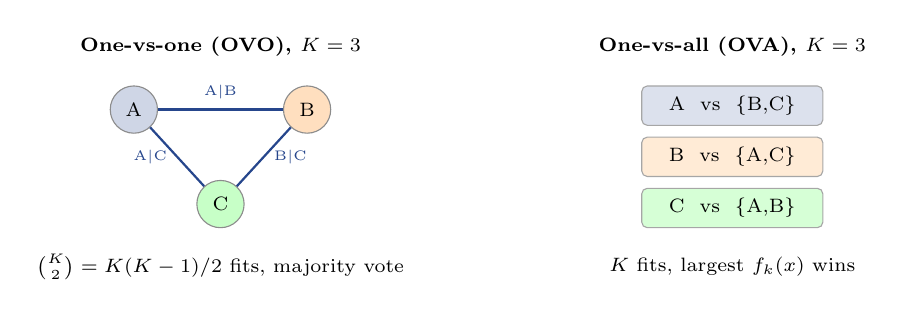
\begin{tikzpicture}[font=\scriptsize,
      cls/.style={circle,draw=black!45,minimum size=6mm,inner sep=1pt},
      bx/.style={draw=black!35,rounded corners=2pt,minimum width=2.3cm,minimum height=5mm,align=center,font=\scriptsize}]
    \node[font=\bfseries\scriptsize] at (1.7,1.9) {One-vs-one (OVO), $K=3$};
    \node[cls,fill=accent!22]  (a) at (0.6,1.1) {A};
    \node[cls,fill=orange!25]  (b) at (2.8,1.1) {B};
    \node[cls,fill=green!22]   (c) at (1.7,-0.1) {C};
    \draw[thick,accent] (a)--(b) node[midway,above,font=\tiny]{A$|$B};
    \draw[thick,accent] (a)--(c) node[midway,left,font=\tiny]{A$|$C};
    \draw[thick,accent] (b)--(c) node[midway,right,font=\tiny]{B$|$C};
    \node at (1.7,-0.9) {$\binom{K}{2}=K(K-1)/2$ fits, majority vote};
    \node[font=\bfseries\scriptsize] at (8.2,1.9) {One-vs-all (OVA), $K=3$};
    \node[bx,fill=accent!16]  at (8.2,1.15) {A \ vs \ \{B,C\}};
    \node[bx,fill=orange!16]  at (8.2,0.5) {B \ vs \ \{A,C\}};
    \node[bx,fill=green!16]   at (8.2,-0.15) {C \ vs \ \{A,B\}};
    \node at (8.2,-0.9) {$K$ fits, largest $f_k(x)$ wins};
  \end{tikzpicture}
  \end{center}
  \begin{takeaway}
    \texttt{SVC} uses \textbf{OVO}; \texttt{LinearSVC} uses OVA. Neither is a
    principled multi-class objective --- both are \emph{voting schemes} bolted
    onto a binary method, and they can disagree. OVO's votes can tie; OVA
    compares scores from models fitted on different, badly unbalanced problems.
  \end{takeaway}
\end{frame}

\begin{frame}{Exercise 9.7 --- Counting multi-class classifiers [Concept]}
\begin{exercise}
  \begin{enumerate}
    \item How many binary classifiers do OVO and OVA need for $K=4$? For
          $K=10$?
    \item With $K=10$ balanced classes and $n=10\,000$, how many observations
          does one OVO fit use, and how many does one OVA fit use?
    \item Kernel SVM training cost grows roughly like the square of the
          training-set size. Which scheme does less total work at $K=10$?
    \item Name one respect in which OVA is nonetheless the more honest
          construction.
  \end{enumerate}
\end{exercise}
\end{frame}

\begin{frame}{Solution --- Exercise 9.7}
\begin{solutionbox}
  \scriptsize
  \textbf{Part 1.} OVO needs $\binom{K}{2}=K(K-1)/2$: $\binom{4}{2}=6$ and
  $\binom{10}{2}=45$. OVA needs $K$: $4$ and $10$.

  \textbf{Part 2.} Balanced classes give $n/K = 1\,000$ per class. An OVO fit
  sees two classes, so $2\,000$ observations; an OVA fit sees all $10\,000$.

  \textbf{Part 3.} With cost $\propto m^2$ in the sub-sample size $m$:
  \[
    \text{OVO: } 45 \times 2\,000^2 = 1.8\times10^{8},
    \qquad
    \text{OVA: } 10 \times 10\,000^2 = 1.0\times10^{9} .
  \]
  OVO does about $5.6$ times \emph{less} work despite fitting $4.5$ times as
  many models --- which is why \texttt{SVC} defaults to it.

  \textbf{Part 4.} OVA produces exactly one score $f_k(x)$ per class, so the
  prediction is a single $\arg\max$ with no ties and no vote-counting, and each
  fit answers a question we care about (``is it class $k$?''). Its weakness
  mirrors OVO's: each fit is badly unbalanced ($1$ against $9$), and the $K$
  scores are not on a comparable scale.
\end{solutionbox}
\end{frame}

% ============================================================
\section{Tuning and Comparison}
% ============================================================

\begin{frame}{Tuning $C$ and $\gamma$ by cross-validation (bridge to Chapter 5)}
  \footnotesize
  \begin{block}{The recipe}
    \begin{enumerate}
      \item Put \texttt{StandardScaler} and \texttt{SVC} in a
            \texttt{Pipeline}, so scaling is refitted inside every fold.
      \item Lay out a \emph{logarithmic} grid, e.g.\
            $C\in\{10^{-2},\dots,10^{2}\}$, $\gamma\in\{10^{-4},\dots,10^{0}\}$.
      \item Score every cell by $k$-fold CV on the \textbf{training} data only.
      \item Refit the winning cell on all the training data; report on the
            untouched test set.
    \end{enumerate}
  \end{block}
  \begin{readme}
    \begin{itemize}
      \item Grids must be logarithmic: $C$ and $\gamma$ act multiplicatively,
            so $\{1,2,3\}$ explores almost nothing.
      \item If the winner sits on the edge of the grid, extend the grid --- the
            optimum is outside it.
      \item Nested CV if you also want an honest error estimate for the
            \emph{tuned} model; one held-out test set is the cheap version.
    \end{itemize}
  \end{readme}
\end{frame}

\begin{frame}{The $(C,\gamma)$ surface on the Heart data}
  \begin{center}
    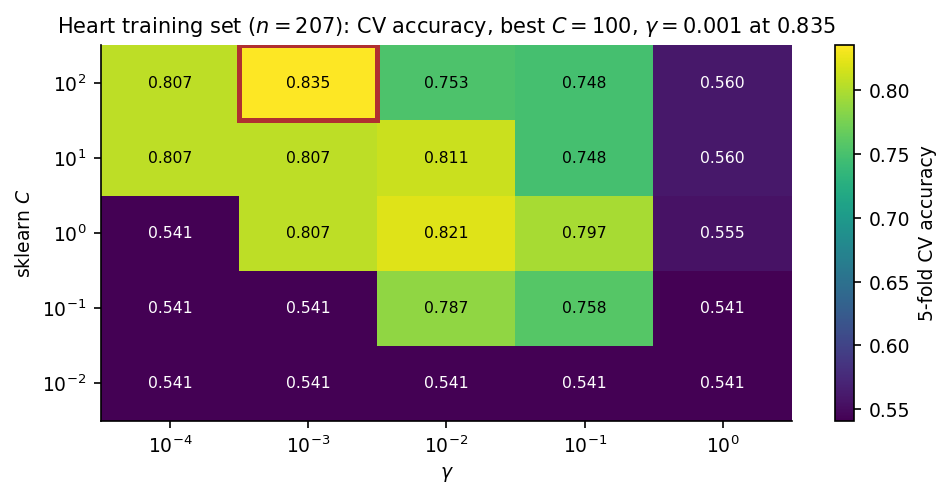
\includegraphics[width=0.62\textwidth,height=0.46\textheight,keepaspectratio]{ch09_cv_heatmap.png}
  \end{center}
  \begin{takeaway}
    The best cell is $C=100$, $\gamma=10^{-3}$ at CV accuracy $0.835$. The dark
    cells at $0.541$ are exactly the training-set majority-class rate: there the
    model has degenerated to ``always predict No''. Note the diagonal ridge ---
    large $\gamma$ needs small $C$ and vice versa, which is why they must be
    tuned together.
  \end{takeaway}
\end{frame}

\begin{frame}{Flexibility is not free: $\gamma$ and the test set}
  \begin{center}
    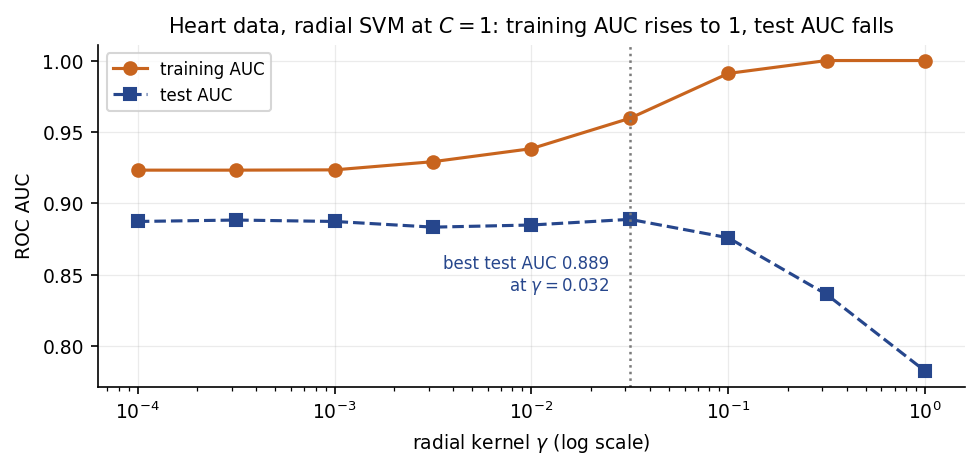
\includegraphics[width=0.78\textwidth,height=0.48\textheight,keepaspectratio]{ch09_heart_gamma_auc.png}
  \end{center}
  \begin{takeaway}
    At $C=1$, raising $\gamma$ drives training AUC from $0.923$ to a perfect
    $1.000$ while test AUC \emph{falls} from $0.887$ to $0.782$. The best test
    AUC, $0.889$, comes at $\gamma\approx0.03$ --- a boundary barely more
    flexible than a straight line.
  \end{takeaway}
\end{frame}

\begin{frame}{SVM vs.\ logistic regression: the honest comparison is the loss}
  \footnotesize
  \begin{block}{Both minimise ``loss $+$ ridge penalty''}
    \[
      \boxed{\;
      \min_{\beta_0,\beta}\ \sum_{i=1}^{n} L\big(y_i f(x_i)\big) + \lambda\|\beta\|^2,
      \quad
      L(t) = \max\{0,\,1-t\}\ \text{(hinge, SVM)}
      \ \text{ or }\
      \log\!\big(1+e^{-t}\big)\ \text{(logistic)}\;}
    \]
  \end{block}
  \begin{readme}
    \begin{itemize}
      \item $t = y_i f(x_i)$ is the functional margin; $\lambda = 1/(2C)$ ties
            the penalty back to sklearn's $C$.
      \item The \textbf{hinge} loss is \emph{exactly zero} for $t\ge1$, so
            points comfortably right contribute nothing --- that is the
            sparsity, and the support vectors, in one line.
      \item The \textbf{logistic} loss is never zero, so \emph{every}
            observation nudges the fit, a little, forever.
    \end{itemize}
  \end{readme}
  \begin{takeaway}
    Same linear model, same ridge penalty, different loss. That is the whole
    difference --- not ``geometry versus probability''.
  \end{takeaway}
\end{frame}

\begin{frame}{Hinge and logistic loss, drawn}
  \begin{center}
    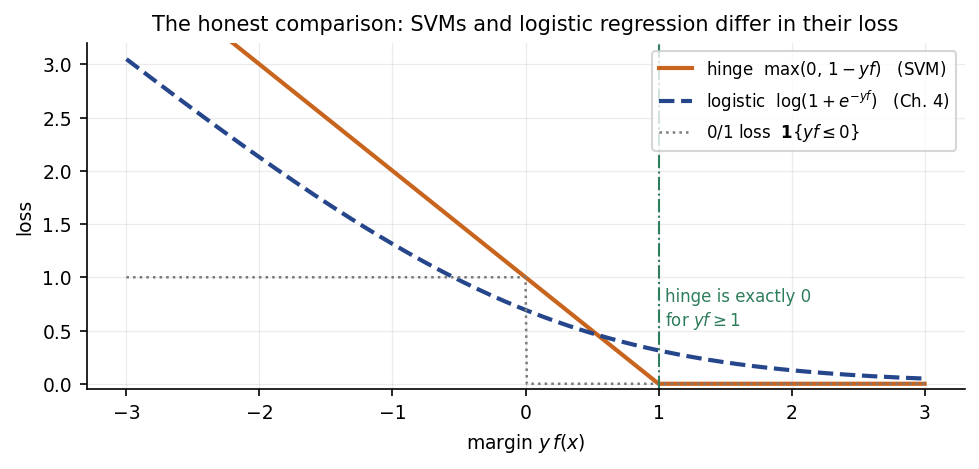
\includegraphics[width=0.82\textwidth,height=0.48\textheight,keepaspectratio]{ch09_losses.png}
  \end{center}
  \begin{takeaway}
    Both are convex upper bounds on the $0/1$ loss and nearly coincide near
    $t=0$ --- which is why the two methods usually agree. They differ at the
    ends: hinge switches off at $t=1$ (sparsity), logistic keeps a tail
    (probabilities, and sensitivity to far-away points).
  \end{takeaway}
\end{frame}

\begin{frame}{SVMs give you no probabilities}
  \footnotesize
  \begin{readme}[{{What you get, and what you do not}}]
    \begin{itemize}
      \item \texttt{decision\_function(X)} returns $f(x)$: a real-valued,
            monotone \emph{score}. That is all an ROC curve or an AUC needs, so
            Chapter 4's ranking machinery still applies.
      \item \texttt{predict\_proba} does not exist unless you pass
            \texttt{SVC(probability=True)}, which fits a \textbf{separate}
            logistic calibration (Platt scaling) by internal 5-fold CV.
    \end{itemize}
  \end{readme}
  \begin{mistake}
    Using \texttt{SVC(probability=True).predict\_proba(...)[:,1]} for an ROC
    curve. On the Heart data it happens to give the identical AUC ($0.899$;
    Spearman correlation $1.00$ with $f$), but it is a different estimator,
    seeded, and several times slower to fit. \textbf{For ROC and AUC, always
    use \texttt{decision\_function}.}
  \end{mistake}
  \begin{takeaway}
    Need calibrated probabilities for an expected-cost decision? Calibrate
    deliberately, or use logistic regression, which gives them for free.
  \end{takeaway}
\end{frame}

\begin{frame}{ROC on the Heart test set: SVM, logistic, forest}
  \begin{center}
    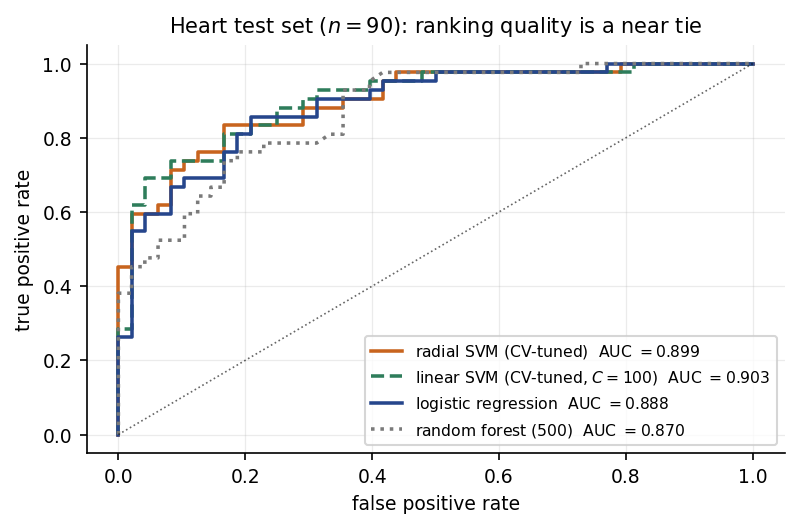
\includegraphics[width=0.50\textwidth,height=0.50\textheight,keepaspectratio]{ch09_roc.png}
  \end{center}
  \begin{takeaway}
    Four methods, $90$ test patients, AUCs within $0.033$: linear SVM $0.903$,
    radial SVM $0.899$, logistic regression $0.888$, random forest $0.870$. The
    \emph{simplest} kernel wins --- the radial one buys nothing here.
  \end{takeaway}
\end{frame}

\begin{frame}{SVM vs.\ trees and forests (bridge to Chapter 8)}
  \scriptsize
  \begin{center}
  \begin{tabular}{@{}p{2.8cm}p{3.2cm}p{3.4cm}p{3.0cm}@{}}
    \toprule
     & \textbf{SVM (radial)} & \textbf{Logistic regression} & \textbf{Random forest} \\
    \midrule
    Boundary shape & smooth, curved & linear in $X$ & axis-aligned steps \\
    Probabilities & none by default & yes & yes, from vote shares \\
    Needs scaling & \textbf{yes, essential} & helpful for penalties & no \\
    Categoricals & must be encoded & must be encoded & handled natively \\
    $p \gg n$ & very strong & needs a penalty & workable \\
    Missing values & must be imputed & must be imputed & tolerant \\
    Interpretation & weak & coefficients, odds ratios & importances \\
    Tuning burden & $C$, $\gamma$, kernel & little & moderate \\
    Heart test AUC & $0.899$ & $0.888$ & $0.870$ \\
    \bottomrule
  \end{tabular}
  \end{center}
  \begin{takeaway}
    On $297$ patients with $16$ mixed predictors all three land inside $0.03$
    AUC of each other. Choose on the \emph{secondary} criteria ---
    probabilities, interpretability, missing data, tuning cost --- because
    accuracy will not decide it for you.
  \end{takeaway}
\end{frame}

\begin{frame}{When to reach for an SVM}
  \footnotesize
  \begin{readme}[Decision guidance]
    \begin{itemize}
      \item \textbf{Reach for it} when $p$ is large relative to $n$, when the
            classes are close to separable, when a bespoke similarity (string,
            graph, sequence kernel) is natural, or when you need a hard,
            reproducible boundary.
      \item \textbf{Reach elsewhere} when you need probabilities, when $n$ is
            in the hundreds of thousands ($n\times n$ kernel matrices do not
            fit), when the data are mostly categorical with missing values, or
            when a stakeholder must read coefficients.
    \end{itemize}
  \end{readme}
  \begin{takeaway}[Why the SVM never became the default]
    Credit scorecards must give a monotone, explainable probability of default
    and survive a regulator asking ``why was this applicant declined?'';
    penalised logistic regression and boosted trees with SHAP answer that, a
    radial-kernel SVM does not. The method stayed where explanation matters
    less and $p/n$ is brutal --- assays, spectra, text, novelty detection.
  \end{takeaway}
\end{frame}

% ------------------------------------------------------------
% EXTENDED EXERCISE 9.2
\begin{frame}{Extended Exercise 9.2 --- Tune an SVM on Heart and race it [Python]}
\begin{longexercise}
  Using the Heart split of Exercise 9.6 ($207$ train, $90$ test):
  \begin{enumerate}
    \item In a scaled \texttt{Pipeline}, tune a radial SVM by 5-fold CV over
          $C\in\{10^{-2},\dots,10^{2}\}$ and
          $\gamma\in\{10^{-4},\dots,10^{0}\}$ (five values each). Report the
          best cell, its CV and test accuracy, and its number of support
          vectors.
    \item Do the same for a \emph{linear} kernel over the same $C$ grid.
    \item Fit a scaled logistic regression and a $500$-tree random forest.
    \item Report the test ROC AUC of all four, using
          \texttt{decision\_function} for the SVMs and
          \texttt{predict\_proba} for the others. Which wins, and by how much?
    \item What do you conclude about the value of the radial kernel here?
  \end{enumerate}
\end{longexercise}
\begin{labnote}[Run this live]
  Worked in \texttt{advanced\_05\_svm\_lab.ipynb} under \emph{Lecture exercises
  --- worked Python solutions}: \emph{Extended Exercise 9.2}.
\end{labnote}
\end{frame}

\begin{frame}[fragile]{Solution --- Extended Exercise 9.2 (1/2)}
\begin{solutionbox}[Solution --- code]
\begin{lstlisting}[basicstyle=\ttfamily\tiny]
Cs = np.array([0.01, 0.1, 1.0, 10.0, 100.0])            # log grid, 5 values
Gs = np.array([1e-4, 1e-3, 1e-2, 1e-1, 1.0])            # log grid, 5 values
pipe = lambda **kw: make_pipeline(StandardScaler(), SVC(**kw))  # scale in-fold
rbf = GridSearchCV(pipe(kernel='rbf'),
                   {'svc__C': Cs, 'svc__gamma': Gs}, cv=5).fit(Xtr, ytr)  # 25 cells
lin = GridSearchCV(pipe(kernel='linear'), {'svc__C': Cs}, cv=5).fit(Xtr, ytr)
for nm, gs in [('radial', rbf), ('linear', lin)]:   # report both fits
    print(nm, gs.best_params_, 'CV', round(gs.best_score_, 3),
          'test', round(gs.score(Xte, yte), 3),
          'nSV', gs.best_estimator_[-1].n_support_.sum())  # 80 vs 72

lg = make_pipeline(StandardScaler(), LogisticRegression(max_iter=5000)).fit(Xtr, ytr)
rf = RandomForestClassifier(n_estimators=500, random_state=0).fit(Xtr, ytr)
scores = {'radial SVM': rbf.best_estimator_.decision_function(Xte),  # NOT proba
          'linear SVM': lin.best_estimator_.decision_function(Xte),
          'logistic':   lg.predict_proba(Xte)[:, 1],  # a real probability
          'forest':     rf.predict_proba(Xte)[:, 1]}  # vote share, 500 trees
for nm, sc in scores.items():                            # roc_auc_score
    print('%-11s AUC=%.3f' % (nm, roc_auc_score(yte, sc)))  # order is all it needs
\end{lstlisting}
{\scriptsize\textbf{Reading it:} both SVMs are tuned on the training split;
all four are then compared by AUC on the test split.}
\end{solutionbox}
\end{frame}

\begin{frame}{Solution --- Extended Exercise 9.2 (2/2)}
\begin{solutionbox}[{{Solution --- output, and what it means}}]
  \scriptsize
  \textbf{Printout.}
  \begin{center}\ttfamily\tiny
  radial \{'svc\_\_C': 100.0, 'svc\_\_gamma': 0.001\} CV 0.835 test 0.789 nSV 80\\
  linear \{'svc\_\_C': 100.0\} CV 0.84 test 0.822 nSV 72\\[2pt]
  radial SVM \ AUC=0.899 \quad linear SVM \ AUC=0.903 \quad
  logistic \ \ AUC=0.888 \quad forest \ \ \ AUC=0.870
  \end{center}
  \begin{itemize}
    \item \textbf{(1)--(2)} The tuned radial kernel picks $\gamma=10^{-3}$, so
          small that the kernel is \emph{nearly linear}: CV has itself told us
          the extra flexibility is unwanted.
    \item \textbf{(4)} All four AUCs lie in $[0.870,\,0.903]$ --- a spread of
          $0.033$ on $90$ test patients, inside sampling noise at this size.
    \item \textbf{(5)} The radial kernel buys \emph{nothing}: the linear SVM is
          at least as good on CV accuracy ($0.840$ vs.\ $0.835$) and test AUC
          ($0.903$ vs.\ $0.899$), with fewer support vectors and one
          hyperparameter instead of two. Prefer it.
  \end{itemize}
\end{solutionbox}
\begin{mistake}
  Reading the winner of a $0.033$ AUC gap on $n=90$ as a real finding. Quote
  the spread, or bootstrap a confidence interval, before declaring a champion.
\end{mistake}
\end{frame}

% ============================================================
\section{Python Lab}
% ============================================================

\begin{frame}{Python lab --- run it live in the notebook}
  \begin{labnote}[{Companion notebook: \texttt{advanced\_05\_svm\_lab.ipynb}}]
    The code in this section is meant to be \textbf{demonstrated live}. Open
    the companion Jupyter notebook and run it cell by cell:
    \begin{itemize}
      \item \S1, \emph{Synthetic two-class data} --- the concentric rings from
            \texttt{make\_circles};
      \item \S2, \emph{Linear SVM} --- the margin, the support vectors and
            sklearn's $C$;
      \item \S3, \emph{Radial-kernel SVM} --- $\gamma$, and the decision
            boundaries side by side;
      \item \S4, \emph{Real data: Heart} --- encoding, scaling, and the
            unscaled disaster;
      \item \S5, \emph{Tuning $C$ and $\gamma$ by cross-validation} --- the
            grid, the heatmap and the ROC race.
    \end{itemize}
    Data loads via the \texttt{ISLP} package or the bundled CSV files;
    \S6, \emph{Exercises} ends the notebook with hands-on tasks.
  \end{labnote}
\end{frame}

\begin{frame}[fragile]{A support vector classifier from start to finish}
  \begin{lstlisting}[basicstyle=\ttfamily\scriptsize]
import numpy as np
from sklearn.pipeline import make_pipeline           # scaler + model as one
from sklearn.preprocessing import StandardScaler     # SVMs NEED this
from sklearn.svm import SVC                          # large C = narrow street

rng = np.random.default_rng(2024)                    # seeded: reproducible
X = rng.normal(size=(20, 2))                         # 20 points in the plane
y = np.repeat([-1, 1], 10)                           # +-1 labels, 10 each
X[y == 1] += 2.5                                     # now separable by a line

hard = SVC(kernel='linear', C=1e6).fit(X, y)         # huge C ~ hard margin
print('n support vectors:', hard.n_support_.sum())   # 3 of 20 shape the fit
print('margin 1/||beta|| :', round(1 / np.linalg.norm(hard.coef_), 3))  # 0.369
  \end{lstlisting}
  \begin{takeaway}
    \texttt{C=1e6} is how you ask \texttt{SVC} for a (near) hard margin ---
    remember, \emph{large} sklearn $C$ means \emph{narrow} margin.
  \end{takeaway}
\end{frame}

\begin{frame}[fragile]{A radial-kernel SVM, tuned, and its ROC score}
  \begin{lstlisting}[basicstyle=\ttfamily\scriptsize]
from sklearn.datasets import make_circles            # rings, not separable
from sklearn.metrics import roc_auc_score            # ranks, not labels
from sklearn.model_selection import GridSearchCV     # refits on the best cell

X, y = make_circles(n_samples=300, factor=0.4, noise=0.15, random_state=0)
grid = {'svc__C': np.logspace(-2, 2, 5),             # log grid, 5 x 5 cells
        'svc__gamma': np.logspace(-3, 1, 5)}         # gamma: locality
gs = GridSearchCV(make_pipeline(StandardScaler(), SVC(kernel='rbf')),
                  grid, cv=5).fit(X, y)              # scaling inside each fold
print('best:', gs.best_params_, 'CV:', round(gs.best_score_, 3))  # C=1, g=10

s = gs.best_estimator_.decision_function(X)          # no predict_proba needed
print('in-sample AUC:', round(roc_auc_score(y, s), 3))  # a ranking is enough
  \end{lstlisting}
  \begin{mistake}
    Scaling once outside \texttt{GridSearchCV}: every fold's validation rows
    have then already influenced the mean and variance used to transform them
    --- a small but real leak that flatters the CV score.
  \end{mistake}
\end{frame}

% ============================================================
\section{Summary}
% ============================================================

\begin{frame}{Chapter 9 in one slide}
  \footnotesize
  \begin{block}{What we accomplished}
    Classification as geometry: the widest street between two classes, made
    robust by a budget and made non-linear by a kernel.
  \end{block}
  \begin{itemize}
    \item Separating hyperplanes, the score $f(x)$, the functional margin
          $y_i f(x_i)$.
    \item The maximal margin classifier, $M=1/\|\beta\|$, and its two fatal
          flaws.
    \item The support vector classifier: slacks $\xi_i$, a budget on
          $\sum_i\xi_i$, and sklearn's inverted $C$.
    \item Support vector machines: the kernel trick, degree $d$, and $\gamma$.
    \item One-vs-one and one-vs-all for $K>2$ classes.
    \item Tuning $(C,\gamma)$ by cross-validation; hinge vs.\ logistic loss;
          ROC from \texttt{decision\_function}.
  \end{itemize}
\end{frame}

\begin{frame}{Key formulas at a glance}
  \scriptsize
  \begin{description}
    \item[Hyperplane] $\{x: \beta_0+\beta^\top x = 0\}$; classifier
      $\hat y = \operatorname{sign} f(x)$, $f(x)=\beta_0+\beta^\top x$.
    \item[Signed distance] $f(x_0)/\|\beta\|$; correct classification
      $\iff y_i f(x_i)>0$.
    \item[Maximal margin] $\max M$ s.t.\ $\|\beta\|=1$, $y_i f(x_i)\ge M\ \forall i$.
    \item[Canonical form] $\min \tfrac12\|\beta\|^2$ s.t.\ $y_i f(x_i)\ge 1$, giving $M=1/\|\beta\|$.
    \item[Soft margin (ISLP)] $\max M$ s.t.\ $\|\beta\|=1$, $y_i f(x_i)\ge M(1-\xi_i)$,
      $\xi_i\ge0$, $\sum_{i=1}^n \xi_i \le C_{\text{ISLP}}$.
    \item[Soft margin (sklearn)] $\min \tfrac12\|\beta\|^2 + C\sum_i \xi_i$ s.t.\
      $y_i f(x_i)\ge 1-\xi_i$, $\xi_i\ge0$; slack $\xi_i=\max\{0,1-y_if(x_i)\}$.
    \item[Penalised form] $\min \sum_i \max\{0,1-y_if(x_i)\} + \lambda\|\beta\|^2$, $\lambda = 1/(2C)$.
    \item[Dual / kernel rule] $f(x)=\beta_0+\sum_{i\in\mathcal S}\alpha_i K(x,x_i)$, $\alpha_i\ne0$ only on $\mathcal S$.
    \item[Kernels] linear $\langle x,x'\rangle$; polynomial $(1+\langle x,x'\rangle)^d$;
      radial $\exp(-\gamma\|x-x'\|^2)$.
    \item[Enlarged dimension] $\binom{p+d}{d}$ monomials up to degree $d$
      ($\binom{4}{2}=6$ for $p=d=2$; $\binom{103}{3}=176\,851$ for $p=100$, $d=3$).
    \item[Losses] hinge $\max\{0,1-t\}$ vs.\ logistic $\log(1+e^{-t})$, $t=y_if(x_i)$.
    \item[Multi-class] OVO: $\binom{K}{2}=K(K-1)/2$ fits, majority vote;
      OVA: $K$ fits, $\hat y = \arg\max_k f_k(x)$.
  \end{description}
\end{frame}

\begin{frame}{Vocabulary checklist}
  \scriptsize
  \begin{tabular}{ll}
    \toprule
    \textbf{Term} & \textbf{Meaning} \\
    \midrule
    Hyperplane & Flat $(p-1)$-dimensional boundary $\beta_0+\beta^\top x=0$ \\
    Functional margin & $y_i f(x_i)$; positive iff correctly classified \\
    Margin $M$ & Distance from boundary to nearest point; $1/\|\beta\|$ canonically \\
    Support vector & Observation with $y_i f(x_i)\le1$; the only ones that matter \\
    Slack $\xi_i$ & $\max\{0,1-y_if(x_i)\}$; $>1$ means misclassified \\
    Budget $C_{\text{ISLP}}$ & Cap on $\sum_i\xi_i$; larger $=$ wider margin \\
    sklearn $C$ & Cost per unit slack; larger $=$ \emph{narrower} margin \\
    Support vector classifier & Soft margin with a linear kernel \\
    Support vector machine & Soft margin with a non-linear kernel \\
    Kernel $K(x,x')$ & Inner product in an implicit enlarged space $\phi$ \\
    $\gamma$ & Radial-kernel locality; large $\gamma$ $=$ wiggly boundary \\
    Hinge loss & $\max\{0,1-t\}$; zero once a point is safely right \\
    \texttt{decision\_function} & The score $f(x)$; what ROC curves need \\
    Platt scaling & Post-hoc logistic calibration behind \texttt{probability=True} \\
    OVO / OVA & One-vs-one / one-vs-all multi-class wrappers \\
    \bottomrule
  \end{tabular}
\end{frame}

\begin{frame}{Decision rules of thumb}
  \footnotesize
  \begin{itemize}
    \item \textbf{Always} put a \texttt{StandardScaler} in front of an SVM,
          inside a \texttt{Pipeline}.
    \item Start with a \textbf{linear} kernel; move to radial only if CV says
          the extra flexibility pays.
    \item Tune $C$ and $\gamma$ \emph{jointly} on a logarithmic grid; extend
          the grid if the winner sits on its edge.
    \item Many support vectors $\Rightarrow$ wide margin $\Rightarrow$ high
          bias, low variance. Few $\Rightarrow$ the reverse.
    \item Report ROC AUC from \texttt{decision\_function}; reach for
          \texttt{probability=True} only when you genuinely need probabilities.
    \item $n$ in the hundreds of thousands? Use \texttt{LinearSVC} or
          \texttt{SGDClassifier(loss='hinge')} --- an $n\times n$ kernel matrix
          will not fit.
    \item Must explain a decision to a regulator or a clinician? Prefer
          penalised logistic regression or a boosted tree.
  \end{itemize}
\end{frame}

\begin{frame}{Common pitfalls}
  \footnotesize
  \begin{alertblock}{Don't}
    \begin{enumerate}
      \item Confuse ISLP's budget $C_{\text{ISLP}}$ with sklearn's cost $C$ ---
            they run in \emph{opposite} directions.
      \item Fit an SVM on unscaled predictors, or scale outside the CV loop.
      \item Say ``the budget limits how many points are misclassified''. It
            limits $\sum_i \xi_i$.
      \item Treat many support vectors as a sign of overfitting.
      \item Read $|f(x)|$ as a probability, or as a distance without dividing
            by $\|\beta\|$.
      \item Draw an ROC curve from \texttt{SVC(probability=True)} instead of
            \texttt{decision\_function}.
      \item Tune $\gamma$ and $C$ one at a time, or on a linear grid.
      \item Use \texttt{kernel='poly'} without \texttt{coef0=1} and expect
            ISLP's $(1+\langle x,x'\rangle)^d$.
      \item Declare a winner from a $0.03$ AUC gap on $90$ test observations.
    \end{enumerate}
  \end{alertblock}
\end{frame}

\begin{frame}{Self-check questions}
  \scriptsize
  \begin{readme}[Quick self-assessment]
    \begin{enumerate}
      \item Why does the maximal margin problem impose $\|\beta\|=1$, and what
            replaces that constraint in the form software solves?
      \item An observation has $\xi_i = 0.6$. Is it misclassified? Is it a
            support vector?
      \item You double sklearn's $C$. What happens to the margin, to
            $\|\beta\|$, and to $|\mathcal S|$?
      \item Why can a radial kernel work when its enlarged feature space is
            infinite-dimensional?
      \item Which loss --- hinge or logistic --- is zero for some observations,
            and why does that produce sparsity?
    \end{enumerate}
  \end{readme}
  \begin{takeaway}[Answers]
    (1) To make $y_if(x_i)$ a true distance; the canonical scaling
    $y_if(x_i)\ge1$ replaces it, and then $M=1/\|\beta\|$.
    (2) Not misclassified (that needs $\xi_i>1$), but yes, a support vector.
    (3) Margin narrows, $\|\beta\|$ grows, $|\mathcal S|$ falls.
    (4) Because fitting and prediction touch the data only through the
    $n\times n$ kernel matrix, never through $\phi$.
    (5) Hinge: it is exactly $0$ once $y_if(x_i)\ge1$, so those points drop out
    of the solution and get $\alpha_i=0$.
  \end{takeaway}
\end{frame}

\begin{frame}{Eight things to remember}
  \footnotesize
  \begin{takeaway}[Chapter 9 in eight lines]
    \begin{enumerate}
      \item An SVM is a \emph{boundary}, not a probability model.
      \item Maximising the margin $=$ minimising $\|\beta\|$; $M=1/\|\beta\|$.
      \item Only the support vectors ($y_if(x_i)\le1$) shape the fit.
      \item The soft margin budgets the \textbf{sum} of the slacks.
      \item sklearn's $C$ is \emph{inverse} regularisation: big $C$, narrow
            street.
      \item Kernels buy a huge feature space at the cost of an $n\times n$
            matrix.
      \item $\gamma$ sets locality; scale your predictors or $\gamma$ means
            nothing.
      \item SVM and logistic regression differ only in their loss --- and
            usually agree.
    \end{enumerate}
  \end{takeaway}
  \begin{takeaway}[What's next]
    Chapter 10 stops \emph{choosing} the enlarged features and \emph{learns}
    them instead: a neural network is a stack of adaptive basis functions with a
    linear rule on top.
  \end{takeaway}
\end{frame}

% ============================================================
\appendix
\AtBeginSection[]{}
\section{Appendix: optional and advanced material}
% ============================================================

\begin{frame}{Appendix --- what is in here, and why}
  \scriptsize
  Nothing in the appendix is needed to follow the chapter: each slide is a
  formal derivation, a longer worked exercise, or a side topic. Read it when
  you want the full story, or when a later chapter sends you back here.
  \begin{block}{Contents of the appendix}
    \begin{itemize}
      \item \textbf{The polynomial kernel: what degree $d$ does} --- the degree sweep drawn; Exercise 9.5 reports the same finding numerically (degree 2 scores 0.963 on a circular boundary).
      \item \textbf{A hyperplane in the plane} --- the picture behind
            Exercise 9.1, moved out because the main deck needs the concept,
            not the drawing.
      \item \textbf{Distance to a hyperplane} --- the two-line derivation
            behind $|f(x_0)|/\|\beta\|$, which the main deck simply asserts.
      \item \textbf{Why $M = 1/\|\beta\|$} --- the algebra that turns
            ``maximise the margin'' into ``minimise $\|\beta\|^2$''.
      \item \textbf{The dual problem} --- where the $\alpha_i$ come from and
            why they vanish off the support vectors. This is the machinery
            behind the kernel trick; examinable only at the level of the
            statement.
      \item \textbf{Support vector regression} --- the same idea for a
            quantitative response, with an $\epsilon$-insensitive tube. A side
            topic, outside ISLP Chapter 9's core.
      \item \textbf{Extended Exercise 9.3} --- a design exercise on choosing
            between SVM, logistic regression and a forest. Run it if the
            session has time; it needs no new theory.
    \end{itemize}
  \end{block}
\end{frame}


\begin{frame}{The polynomial kernel: what degree $d$ does}
  \begin{center}
    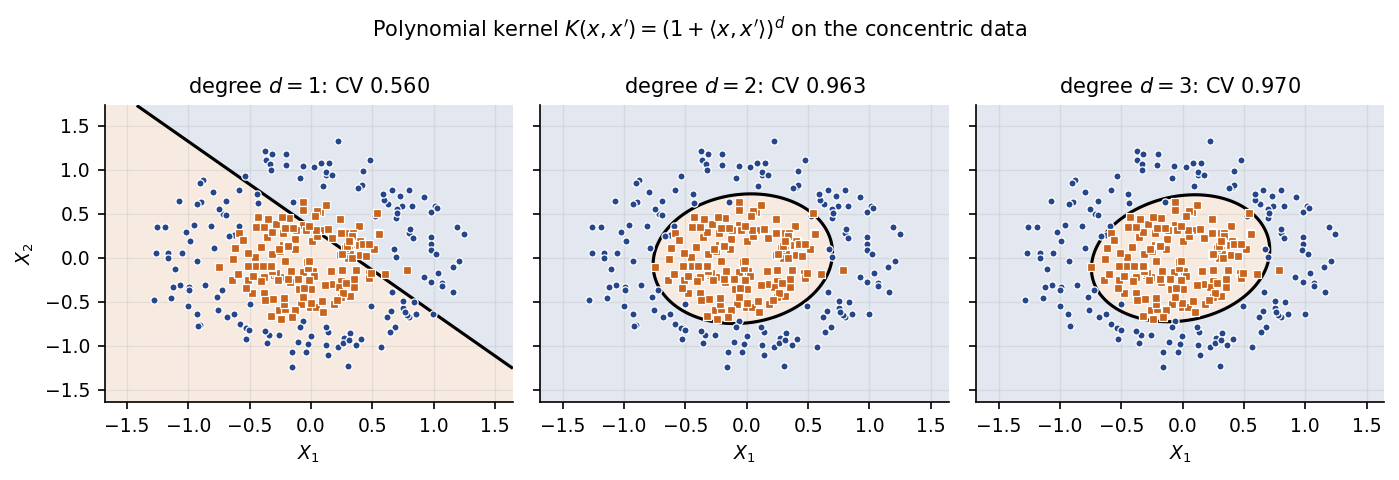
\includegraphics[width=0.90\textwidth,height=0.46\textheight,keepaspectratio]{ch09_poly_degree.png}
  \end{center}
  \begin{takeaway}
    $d=1$ is just a line and scores $0.560$; $d=2$ can bend into an ellipse and
    jumps to $0.963$; $d=3$ reaches $0.970$. Almost all the gain comes from the
    \emph{first} step past linearity, because the true boundary here is a
    circle --- a degree-$2$ shape.
  \end{takeaway}
\end{frame}

\begin{frame}{A hyperplane in the plane}
  \begin{center}
    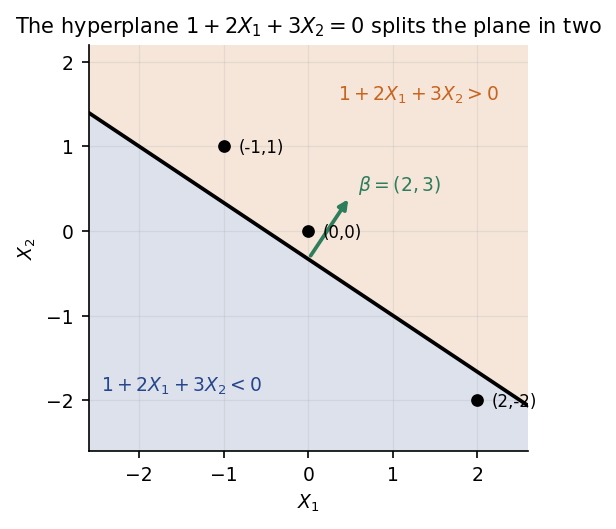
\includegraphics[width=0.54\textwidth,height=0.52\textheight,keepaspectratio]{ch09_hyperplane.png}
  \end{center}
  \begin{takeaway}
    Points with $1+2X_1+3X_2>0$ sit in the orange half-space, points with $<0$
    in the blue one. The green arrow is $\beta=(2,3)$: perpendicular to the
    line, pointing into the positive half-space. The three marked points are
    the ones classified in Exercise 9.1.
  \end{takeaway}
\end{frame}

\begin{frame}{Distance from a point to a hyperplane}
  \footnotesize
  \begin{center}
    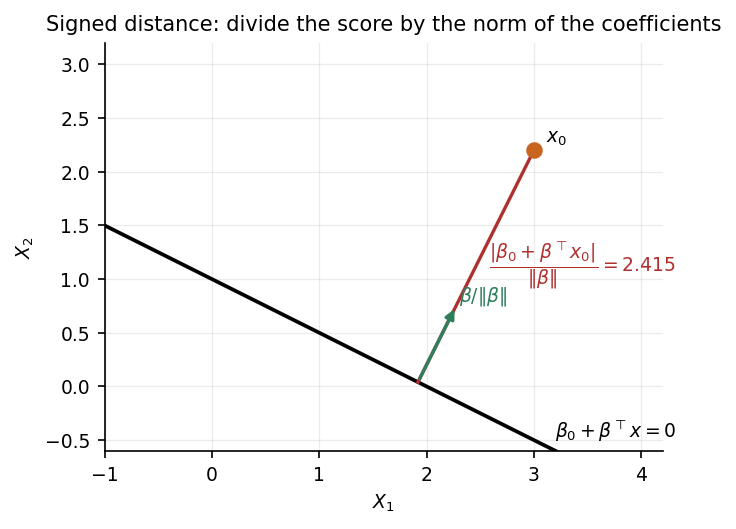
\includegraphics[width=0.56\textwidth,height=0.36\textheight,keepaspectratio]{ch09_x_margin_geometry.png}
  \end{center}
  \begin{readme}[The derivation]
    Let $x_p$ be any point on the plane, so $\beta_0+\beta^\top x_p=0$, and let
    $u = \beta/\|\beta\|$ be the unit normal. The distance from $x_0$ to the
    plane is the length of the projection of $x_0-x_p$ onto $u$:
    \[
      u^\top(x_0-x_p)
      = \frac{\beta^\top x_0 - \beta^\top x_p}{\|\beta\|}
      = \frac{\beta^\top x_0 + \beta_0}{\|\beta\|}
      = \frac{f(x_0)}{\|\beta\|},
    \]
    using $\beta^\top x_p = -\beta_0$. The absolute value is the distance; the
    sign says which side.
  \end{readme}
\end{frame}

\begin{frame}{Why $M = 1/\|\beta\|$}
  \footnotesize
  \begin{readme}[From ``maximise $M$'' to ``minimise $\|\beta\|^2$'']
    \begin{itemize}
      \item Suppose $y_i f(x_i)\ge M$ for all $i$ with $\|\beta\|=1$. By the
            previous slide, $M$ is then the smallest distance from the plane to
            a data point.
      \item Now drop $\|\beta\|=1$ and rescale $(\beta_0,\beta)$ by $1/M$. The
            constraints become $y_i f(x_i)\ge 1$, and the new coefficient
            vector has norm $\|\beta\|_{\text{new}} = 1/M$.
      \item So maximising $M$ over unit-norm $\beta$ is exactly minimising
            $\|\beta\|$ subject to $y_i f(x_i)\ge1$, with $M = 1/\|\beta\|$
            recovered at the end.
      \item Squaring and halving --- minimise $\tfrac12\|\beta\|^2$ --- leaves
            the minimiser unchanged and makes the objective a smooth quadratic,
            which is what QP solvers want.
    \end{itemize}
  \end{readme}
  \begin{takeaway}
    This is why the chapter can be read as ridge regression with a different
    loss: the SVM's primary objective \emph{is} a penalty on $\|\beta\|^2$.
  \end{takeaway}
\end{frame}

\begin{frame}{The dual problem, and where the $\alpha_i$ come from}
  \footnotesize
  \begin{block}{Wolfe dual of the soft-margin problem}
    \[
      \max_{a}\ \sum_{i=1}^n a_i - \tfrac12\sum_{i=1}^n\sum_{i'=1}^n
        a_i a_{i'} y_i y_{i'} K(x_i,x_{i'})
      \quad\text{s.t.}\quad
      0 \le a_i \le C,\quad \sum_{i=1}^n a_i y_i = 0
    \]
  \end{block}
  \begin{readme}
    \begin{itemize}
      \item Write $\alpha_i = a_i y_i$; then
            $f(x)=\beta_0+\sum_i \alpha_i K(x,x_i)$, the rule from the main
            deck. The data appear \emph{only} inside $K(x_i,x_{i'})$ --- that is
            the whole content of the kernel trick.
      \item Complementary slackness gives three cases: $a_i=0$ (outside the
            street, $y_if(x_i)>1$), $0<a_i<C$ (exactly on the kerb), $a_i=C$
            (inside the street or misclassified).
      \item So $a_i=0$ off the support vectors: sparsity is a
            \emph{consequence} of the hinge loss's flat region, not an
            assumption --- and the geometric, mechanical and algebraic
            descriptions of a support vector are one reading of these same
            conditions.
    \end{itemize}
  \end{readme}
\end{frame}

\begin{frame}{Support vector regression (side topic)}
  \footnotesize
  \begin{center}
    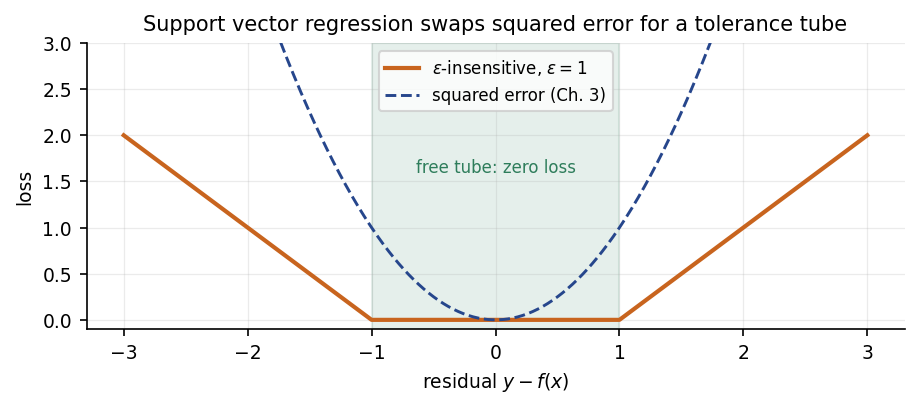
\includegraphics[width=0.58\textwidth,height=0.32\textheight,keepaspectratio]{ch09_x_svr.png}
  \end{center}
  \begin{readme}[The $\epsilon$-insensitive loss]
    Replace the hinge loss by $L_\epsilon(r)=\max\{0,\,|r|-\epsilon\}$ on the
    residual $r=y-f(x)$ and keep the $\|\beta\|^2$ penalty. Residuals inside
    the tube of width $2\epsilon$ cost \emph{nothing}, so again only points on
    or outside the tube become support vectors. In scikit-learn this is
    \texttt{SVR}, with \texttt{epsilon} plus the same \texttt{C}, \texttt{gamma}.
  \end{readme}
  \begin{takeaway}
    Same three ingredients as the classifier --- a flat-bottomed loss, a ridge
    penalty, a kernel --- and the same sparsity. Robust to outliers in a way
    squared error is not, but it too returns no uncertainty.
  \end{takeaway}
\end{frame}

% ------------------------------------------------------------
% EXTENDED EXERCISE 9.3 (appendix)
\begin{frame}{Extended Exercise 9.3 --- Choosing a classifier [Integrative]}
\begin{longexercise}
  For each brief, choose between a radial-kernel SVM, penalised logistic
  regression and a random forest. Justify the choice with this chapter's
  criteria (scaling, $p$ versus $n$, probabilities, missing data,
  interpretability, tuning cost), and name the one thing that would change your
  mind.
  \begin{enumerate}
    \item \textbf{A} --- A proteomics assay: $n=90$ patients, $p=3\,000$ peak
          intensities on a comparable continuous scale, no missing values. The
          output is a two-class research finding.
    \item \textbf{B} --- A consumer credit decision: $n=400\,000$
          applications, $p=45$ mixed numeric and categorical predictors with
          missing income, and a regulator who asks why an applicant was
          declined. An expected-loss calculation needs $\Pr(\text{default})$.
    \item \textbf{C} --- A factory novelty detector: $n=12\,000$ vibration
          traces, $p=60$ engineered spectral features, almost all traces
          normal, and the alarm threshold set later by operations.
  \end{enumerate}
\end{longexercise}
\end{frame}

\begin{frame}{Solution --- Extended Exercise 9.3 (1/2)}
\begin{solutionbox}[{Solution --- briefs A and B}]
  \scriptsize
  \textbf{A --- an SVM, starting linear.} $p/n = 33$, so the data are certainly
  separable: unpenalised logistic regression will not converge, and a forest
  has little to split on with $90$ rows. The margin is well defined even here,
  the features are already on one scale (standardise anyway), and the kernel
  matrix is $90\times90$ --- free. Start \emph{linear}: with $p\gg n$ a linear
  kernel is usually as good as radial and has one hyperparameter.
  \emph{What would change my mind:} if the finding needed a per-patient
  probability for a clinical decision, switch to penalised logistic regression.

  \textbf{B --- penalised logistic regression} (or a boosted tree with SHAP).
  Three deal-breakers for the SVM: $n=400\,000$ makes an $n\times n$ kernel
  matrix impossible ($1.6\times10^{11}$ entries); the decision needs a
  calibrated $\Pr(\text{default})$, which an SVM does not give; and adverse
  action notices need per-applicant reason codes, which coefficients supply and
  support vectors do not. Missing income and categorical predictors also favour
  the GLM/tree side. \emph{What would change my mind:} nothing about the model
  class --- though at $n=4\,000$ instead, \texttt{LinearSVC} would at least be
  feasible.
\end{solutionbox}
\end{frame}

\begin{frame}{Solution --- Extended Exercise 9.3 (2/2)}
\begin{solutionbox}[{{Solution --- brief C, and the common thread}}]
  \scriptsize
  \textbf{C --- an SVM, specifically a one-class SVM.} ``Almost all traces
  normal'' means the negative class is barely observed, so a two-class
  classifier is the wrong framing: fit the \emph{support} of the normal class
  and flag what falls outside. All $60$ features are continuous, so scaling is
  straightforward, and a $12\,000\times12\,000$ kernel matrix is large but
  tractable. Crucially, operations sets the threshold \emph{later}, so a
  monotone score from \texttt{decision\_function} is exactly the right
  deliverable --- no probability needed. \emph{What would change my mind:} once
  enough labelled faults accumulate, a supervised gradient-boosted model would
  probably overtake it.

  \textbf{The common thread.} The SVM wins where $p/n$ is hostile, where the
  deliverable is a \emph{score} rather than a probability, and where a bespoke
  similarity is natural. It loses where $n$ is huge, where probabilities are
  contractual, and where a human must be told why.
\end{solutionbox}
\begin{mistake}
  Choosing on cross-validated accuracy alone. In all three briefs the binding
  constraints are computational and institutional; accuracy is the tie-breaker,
  not the criterion.
\end{mistake}
\end{frame}

\end{document}
